\documentclass[11pt]{article}

% Shared notes settings for Applied Machine Learning lectures (UPES).
% Keep this file free of \documentclass to allow reuse via \input.

\usepackage[utf8]{inputenc}
\usepackage[T1]{fontenc}
\usepackage{lmodern}          % scalable T1 fonts; without this pdflatex falls back
\input{glyphtounicode}        % to bitmapped EC Type 3 and the PDFs are neither
\pdfgentounicode=1            % searchable nor screen-reader friendly
\usepackage[a4paper,margin=1in]{geometry}
\usepackage{hyperref}
\usepackage{xurl}
\usepackage{booktabs}
\usepackage{amsmath}
\usepackage{amssymb}
\usepackage{listings}
\usepackage{xcolor}
\usepackage{enumitem}
\usepackage{parskip}

% Code listings (Python-oriented for this subject).
\lstset{
  language=Python,
  basicstyle=\ttfamily\small,
  keywordstyle=\color{blue},
  commentstyle=\color{gray},
  stringstyle=\color{teal},
  showstringspaces=false,
  columns=fullflexible,
  frame=single,
  framerule=0.2pt,
  breaklines=true
}

\setlist[itemize]{topsep=0.3em,itemsep=0.2em}
\setlist[enumerate]{topsep=0.3em,itemsep=0.2em}

% Simple per-section source line.
\newcommand{\notesources}[1]{\par\noindent{\small\color{gray}\textit{Sources:} \sloppy #1\par}}

% Unit-wise source strings for this subject (used by slides + notes).
% Path is relative to the lecture `latex/` folder (the compilation CWD).
\IfFileExists{../../../_shared/aml-sources.tex}{%
  % Source strings for Applied Machine Learning (CSAI2017P) — used by slides + notes.
% Prescribed texts and reference books are taken from the course syllabus.
% Support texts are the author-hosted open-access editions:
%   statlearning.com            (ISL with Python)
%   probml.github.io/pml-book   (Murphy, Probabilistic Machine Learning)
%   d2l.ai                      (Dive into Deep Learning)
%   mml-book.github.io          (Mathematics for Machine Learning)

\newcommand{\AMLRepoURL}{https://github.com/tali7c/Applied-Machine-Learning}

% --- prescribed -------------------------------------------------------------
\newcommand{\AMLPrescribed}{%
M\"uller and Guido, \textit{Introduction to Machine Learning with Python}, O'Reilly, 2016.;%
Bishop, \textit{Pattern Recognition and Machine Learning}, Springer, 2006.;%
Murphy, \textit{Machine Learning: A Probabilistic Perspective}, MIT Press, 2012.;%
Han, Kamber and Pei, \textit{Data Mining: Concepts and Techniques} (3e), Morgan Kaufmann, 2012.%
}

% --- unit-wise ---------------------------------------------------------------
\newcommand{\AMLUnitISources}{%
M\"uller and Guido, \textit{Introduction to Machine Learning with Python}, Ch. 1.;%
Bishop, \textit{Pattern Recognition and Machine Learning}, Ch. 1.;%
Murphy, \textit{Probabilistic Machine Learning: An Introduction}, MIT Press, 2022, Ch. 1.;%
Mitchell, \textit{Machine Learning}, McGraw Hill, 1997, Ch. 1.;%
Scikit-learn documentation, accessed 2026-08-04.%
}

\newcommand{\AMLUnitIISources}{%
Bishop, \textit{Pattern Recognition and Machine Learning}, \S1.5, \S4.3, \S7.1.;%
Zhang, Lipton, Li and Smola, \textit{Dive into Deep Learning}, \S3.4.;%
Shalev-Shwartz and Ben-David, \textit{Understanding Machine Learning}, Ch. 15.;%
Murphy, \textit{Probabilistic Machine Learning: An Introduction}, Ch. 5.%
}

\newcommand{\AMLUnitIIISources}{%
Zhang, Lipton, Li and Smola, \textit{Dive into Deep Learning}, Ch. 12 (Optimization Algorithms).;%
Deisenroth, Faisal and Ong, \textit{Mathematics for Machine Learning}, Ch. 7.;%
Kingma and Ba, ``Adam: A Method for Stochastic Optimization,'' ICLR 2015.;%
Ruder, ``An overview of gradient descent optimization algorithms,'' arXiv:1609.04747, 2016.%
}

\newcommand{\AMLUnitIVSources}{%
Han, Kamber and Pei, \textit{Data Mining: Concepts and Techniques} (3e), Ch. 3.;%
M\"uller and Guido, \textit{Introduction to Machine Learning with Python}, Ch. 3--4.;%
James, Witten, Hastie, Tibshirani and Taylor, \textit{An Introduction to Statistical Learning with Python}, Ch. 5--6, 12.;%
Scikit-learn documentation (preprocessing, model selection), accessed 2026-08-04.%
}

\newcommand{\AMLUnitVSources}{%
James et al., \textit{An Introduction to Statistical Learning with Python}, Ch. 3--6.;%
Bishop, \textit{Pattern Recognition and Machine Learning}, Ch. 3.;%
Deisenroth, Faisal and Ong, \textit{Mathematics for Machine Learning}, Ch. 9.;%
M\"uller and Guido, \textit{Introduction to Machine Learning with Python}, \S2.3.%
}

\newcommand{\AMLUnitVISources}{%
Han, Kamber and Pei, \textit{Data Mining: Concepts and Techniques} (3e), Ch. 8--9.;%
James et al., \textit{An Introduction to Statistical Learning with Python}, Ch. 8--9.;%
Bishop, \textit{Pattern Recognition and Machine Learning}, Ch. 4--5, 7, 14.;%
Zhang et al., \textit{Dive into Deep Learning}, Ch. 5.%
}

\newcommand{\AMLUnitVIISources}{%
Han, Kamber and Pei, \textit{Data Mining: Concepts and Techniques} (3e), Ch. 10.;%
James et al., \textit{An Introduction to Statistical Learning with Python}, Ch. 12.;%
M\"uller and Guido, \textit{Introduction to Machine Learning with Python}, \S3.5.;%
Ester, Kriegel, Sander and Xu, ``A density-based algorithm for discovering clusters (DBSCAN),'' KDD 1996.%
}

\newcommand{\AMLLabSources}{%
M\"uller and Guido, \textit{Introduction to Machine Learning with Python}, companion notebooks.;%
McKinney, \textit{Python for Data Analysis} (3e), O'Reilly, 2022.;%
Scikit-learn user guide, accessed 2026-08-04.;%
Matplotlib and Seaborn documentation, accessed 2026-08-04.%
}
%
}{%
  % Faculty copies live under `private/` so their compile CWD is different.
  \IfFileExists{../../../../public/_shared/aml-sources.tex}{%
    % Source strings for Applied Machine Learning (CSAI2017P) — used by slides + notes.
% Prescribed texts and reference books are taken from the course syllabus.
% Support texts are the author-hosted open-access editions:
%   statlearning.com            (ISL with Python)
%   probml.github.io/pml-book   (Murphy, Probabilistic Machine Learning)
%   d2l.ai                      (Dive into Deep Learning)
%   mml-book.github.io          (Mathematics for Machine Learning)

\newcommand{\AMLRepoURL}{https://github.com/tali7c/Applied-Machine-Learning}

% --- prescribed -------------------------------------------------------------
\newcommand{\AMLPrescribed}{%
M\"uller and Guido, \textit{Introduction to Machine Learning with Python}, O'Reilly, 2016.;%
Bishop, \textit{Pattern Recognition and Machine Learning}, Springer, 2006.;%
Murphy, \textit{Machine Learning: A Probabilistic Perspective}, MIT Press, 2012.;%
Han, Kamber and Pei, \textit{Data Mining: Concepts and Techniques} (3e), Morgan Kaufmann, 2012.%
}

% --- unit-wise ---------------------------------------------------------------
\newcommand{\AMLUnitISources}{%
M\"uller and Guido, \textit{Introduction to Machine Learning with Python}, Ch. 1.;%
Bishop, \textit{Pattern Recognition and Machine Learning}, Ch. 1.;%
Murphy, \textit{Probabilistic Machine Learning: An Introduction}, MIT Press, 2022, Ch. 1.;%
Mitchell, \textit{Machine Learning}, McGraw Hill, 1997, Ch. 1.;%
Scikit-learn documentation, accessed 2026-08-04.%
}

\newcommand{\AMLUnitIISources}{%
Bishop, \textit{Pattern Recognition and Machine Learning}, \S1.5, \S4.3, \S7.1.;%
Zhang, Lipton, Li and Smola, \textit{Dive into Deep Learning}, \S3.4.;%
Shalev-Shwartz and Ben-David, \textit{Understanding Machine Learning}, Ch. 15.;%
Murphy, \textit{Probabilistic Machine Learning: An Introduction}, Ch. 5.%
}

\newcommand{\AMLUnitIIISources}{%
Zhang, Lipton, Li and Smola, \textit{Dive into Deep Learning}, Ch. 12 (Optimization Algorithms).;%
Deisenroth, Faisal and Ong, \textit{Mathematics for Machine Learning}, Ch. 7.;%
Kingma and Ba, ``Adam: A Method for Stochastic Optimization,'' ICLR 2015.;%
Ruder, ``An overview of gradient descent optimization algorithms,'' arXiv:1609.04747, 2016.%
}

\newcommand{\AMLUnitIVSources}{%
Han, Kamber and Pei, \textit{Data Mining: Concepts and Techniques} (3e), Ch. 3.;%
M\"uller and Guido, \textit{Introduction to Machine Learning with Python}, Ch. 3--4.;%
James, Witten, Hastie, Tibshirani and Taylor, \textit{An Introduction to Statistical Learning with Python}, Ch. 5--6, 12.;%
Scikit-learn documentation (preprocessing, model selection), accessed 2026-08-04.%
}

\newcommand{\AMLUnitVSources}{%
James et al., \textit{An Introduction to Statistical Learning with Python}, Ch. 3--6.;%
Bishop, \textit{Pattern Recognition and Machine Learning}, Ch. 3.;%
Deisenroth, Faisal and Ong, \textit{Mathematics for Machine Learning}, Ch. 9.;%
M\"uller and Guido, \textit{Introduction to Machine Learning with Python}, \S2.3.%
}

\newcommand{\AMLUnitVISources}{%
Han, Kamber and Pei, \textit{Data Mining: Concepts and Techniques} (3e), Ch. 8--9.;%
James et al., \textit{An Introduction to Statistical Learning with Python}, Ch. 8--9.;%
Bishop, \textit{Pattern Recognition and Machine Learning}, Ch. 4--5, 7, 14.;%
Zhang et al., \textit{Dive into Deep Learning}, Ch. 5.%
}

\newcommand{\AMLUnitVIISources}{%
Han, Kamber and Pei, \textit{Data Mining: Concepts and Techniques} (3e), Ch. 10.;%
James et al., \textit{An Introduction to Statistical Learning with Python}, Ch. 12.;%
M\"uller and Guido, \textit{Introduction to Machine Learning with Python}, \S3.5.;%
Ester, Kriegel, Sander and Xu, ``A density-based algorithm for discovering clusters (DBSCAN),'' KDD 1996.%
}

\newcommand{\AMLLabSources}{%
M\"uller and Guido, \textit{Introduction to Machine Learning with Python}, companion notebooks.;%
McKinney, \textit{Python for Data Analysis} (3e), O'Reilly, 2022.;%
Scikit-learn user guide, accessed 2026-08-04.;%
Matplotlib and Seaborn documentation, accessed 2026-08-04.%
}
%
  }{%
    % Question papers live at `private/<family>/<instrument>/`.
    \IfFileExists{../../../public/_shared/aml-sources.tex}{%
      % Source strings for Applied Machine Learning (CSAI2017P) — used by slides + notes.
% Prescribed texts and reference books are taken from the course syllabus.
% Support texts are the author-hosted open-access editions:
%   statlearning.com            (ISL with Python)
%   probml.github.io/pml-book   (Murphy, Probabilistic Machine Learning)
%   d2l.ai                      (Dive into Deep Learning)
%   mml-book.github.io          (Mathematics for Machine Learning)

\newcommand{\AMLRepoURL}{https://github.com/tali7c/Applied-Machine-Learning}

% --- prescribed -------------------------------------------------------------
\newcommand{\AMLPrescribed}{%
M\"uller and Guido, \textit{Introduction to Machine Learning with Python}, O'Reilly, 2016.;%
Bishop, \textit{Pattern Recognition and Machine Learning}, Springer, 2006.;%
Murphy, \textit{Machine Learning: A Probabilistic Perspective}, MIT Press, 2012.;%
Han, Kamber and Pei, \textit{Data Mining: Concepts and Techniques} (3e), Morgan Kaufmann, 2012.%
}

% --- unit-wise ---------------------------------------------------------------
\newcommand{\AMLUnitISources}{%
M\"uller and Guido, \textit{Introduction to Machine Learning with Python}, Ch. 1.;%
Bishop, \textit{Pattern Recognition and Machine Learning}, Ch. 1.;%
Murphy, \textit{Probabilistic Machine Learning: An Introduction}, MIT Press, 2022, Ch. 1.;%
Mitchell, \textit{Machine Learning}, McGraw Hill, 1997, Ch. 1.;%
Scikit-learn documentation, accessed 2026-08-04.%
}

\newcommand{\AMLUnitIISources}{%
Bishop, \textit{Pattern Recognition and Machine Learning}, \S1.5, \S4.3, \S7.1.;%
Zhang, Lipton, Li and Smola, \textit{Dive into Deep Learning}, \S3.4.;%
Shalev-Shwartz and Ben-David, \textit{Understanding Machine Learning}, Ch. 15.;%
Murphy, \textit{Probabilistic Machine Learning: An Introduction}, Ch. 5.%
}

\newcommand{\AMLUnitIIISources}{%
Zhang, Lipton, Li and Smola, \textit{Dive into Deep Learning}, Ch. 12 (Optimization Algorithms).;%
Deisenroth, Faisal and Ong, \textit{Mathematics for Machine Learning}, Ch. 7.;%
Kingma and Ba, ``Adam: A Method for Stochastic Optimization,'' ICLR 2015.;%
Ruder, ``An overview of gradient descent optimization algorithms,'' arXiv:1609.04747, 2016.%
}

\newcommand{\AMLUnitIVSources}{%
Han, Kamber and Pei, \textit{Data Mining: Concepts and Techniques} (3e), Ch. 3.;%
M\"uller and Guido, \textit{Introduction to Machine Learning with Python}, Ch. 3--4.;%
James, Witten, Hastie, Tibshirani and Taylor, \textit{An Introduction to Statistical Learning with Python}, Ch. 5--6, 12.;%
Scikit-learn documentation (preprocessing, model selection), accessed 2026-08-04.%
}

\newcommand{\AMLUnitVSources}{%
James et al., \textit{An Introduction to Statistical Learning with Python}, Ch. 3--6.;%
Bishop, \textit{Pattern Recognition and Machine Learning}, Ch. 3.;%
Deisenroth, Faisal and Ong, \textit{Mathematics for Machine Learning}, Ch. 9.;%
M\"uller and Guido, \textit{Introduction to Machine Learning with Python}, \S2.3.%
}

\newcommand{\AMLUnitVISources}{%
Han, Kamber and Pei, \textit{Data Mining: Concepts and Techniques} (3e), Ch. 8--9.;%
James et al., \textit{An Introduction to Statistical Learning with Python}, Ch. 8--9.;%
Bishop, \textit{Pattern Recognition and Machine Learning}, Ch. 4--5, 7, 14.;%
Zhang et al., \textit{Dive into Deep Learning}, Ch. 5.%
}

\newcommand{\AMLUnitVIISources}{%
Han, Kamber and Pei, \textit{Data Mining: Concepts and Techniques} (3e), Ch. 10.;%
James et al., \textit{An Introduction to Statistical Learning with Python}, Ch. 12.;%
M\"uller and Guido, \textit{Introduction to Machine Learning with Python}, \S3.5.;%
Ester, Kriegel, Sander and Xu, ``A density-based algorithm for discovering clusters (DBSCAN),'' KDD 1996.%
}

\newcommand{\AMLLabSources}{%
M\"uller and Guido, \textit{Introduction to Machine Learning with Python}, companion notebooks.;%
McKinney, \textit{Python for Data Analysis} (3e), O'Reilly, 2022.;%
Scikit-learn user guide, accessed 2026-08-04.;%
Matplotlib and Seaborn documentation, accessed 2026-08-04.%
}
%
    }{%
      % Marking schemes live at `private/solutions/<family>/<id>/latex/`.
      \IfFileExists{../../../../../public/_shared/aml-sources.tex}{%
        % Source strings for Applied Machine Learning (CSAI2017P) — used by slides + notes.
% Prescribed texts and reference books are taken from the course syllabus.
% Support texts are the author-hosted open-access editions:
%   statlearning.com            (ISL with Python)
%   probml.github.io/pml-book   (Murphy, Probabilistic Machine Learning)
%   d2l.ai                      (Dive into Deep Learning)
%   mml-book.github.io          (Mathematics for Machine Learning)

\newcommand{\AMLRepoURL}{https://github.com/tali7c/Applied-Machine-Learning}

% --- prescribed -------------------------------------------------------------
\newcommand{\AMLPrescribed}{%
M\"uller and Guido, \textit{Introduction to Machine Learning with Python}, O'Reilly, 2016.;%
Bishop, \textit{Pattern Recognition and Machine Learning}, Springer, 2006.;%
Murphy, \textit{Machine Learning: A Probabilistic Perspective}, MIT Press, 2012.;%
Han, Kamber and Pei, \textit{Data Mining: Concepts and Techniques} (3e), Morgan Kaufmann, 2012.%
}

% --- unit-wise ---------------------------------------------------------------
\newcommand{\AMLUnitISources}{%
M\"uller and Guido, \textit{Introduction to Machine Learning with Python}, Ch. 1.;%
Bishop, \textit{Pattern Recognition and Machine Learning}, Ch. 1.;%
Murphy, \textit{Probabilistic Machine Learning: An Introduction}, MIT Press, 2022, Ch. 1.;%
Mitchell, \textit{Machine Learning}, McGraw Hill, 1997, Ch. 1.;%
Scikit-learn documentation, accessed 2026-08-04.%
}

\newcommand{\AMLUnitIISources}{%
Bishop, \textit{Pattern Recognition and Machine Learning}, \S1.5, \S4.3, \S7.1.;%
Zhang, Lipton, Li and Smola, \textit{Dive into Deep Learning}, \S3.4.;%
Shalev-Shwartz and Ben-David, \textit{Understanding Machine Learning}, Ch. 15.;%
Murphy, \textit{Probabilistic Machine Learning: An Introduction}, Ch. 5.%
}

\newcommand{\AMLUnitIIISources}{%
Zhang, Lipton, Li and Smola, \textit{Dive into Deep Learning}, Ch. 12 (Optimization Algorithms).;%
Deisenroth, Faisal and Ong, \textit{Mathematics for Machine Learning}, Ch. 7.;%
Kingma and Ba, ``Adam: A Method for Stochastic Optimization,'' ICLR 2015.;%
Ruder, ``An overview of gradient descent optimization algorithms,'' arXiv:1609.04747, 2016.%
}

\newcommand{\AMLUnitIVSources}{%
Han, Kamber and Pei, \textit{Data Mining: Concepts and Techniques} (3e), Ch. 3.;%
M\"uller and Guido, \textit{Introduction to Machine Learning with Python}, Ch. 3--4.;%
James, Witten, Hastie, Tibshirani and Taylor, \textit{An Introduction to Statistical Learning with Python}, Ch. 5--6, 12.;%
Scikit-learn documentation (preprocessing, model selection), accessed 2026-08-04.%
}

\newcommand{\AMLUnitVSources}{%
James et al., \textit{An Introduction to Statistical Learning with Python}, Ch. 3--6.;%
Bishop, \textit{Pattern Recognition and Machine Learning}, Ch. 3.;%
Deisenroth, Faisal and Ong, \textit{Mathematics for Machine Learning}, Ch. 9.;%
M\"uller and Guido, \textit{Introduction to Machine Learning with Python}, \S2.3.%
}

\newcommand{\AMLUnitVISources}{%
Han, Kamber and Pei, \textit{Data Mining: Concepts and Techniques} (3e), Ch. 8--9.;%
James et al., \textit{An Introduction to Statistical Learning with Python}, Ch. 8--9.;%
Bishop, \textit{Pattern Recognition and Machine Learning}, Ch. 4--5, 7, 14.;%
Zhang et al., \textit{Dive into Deep Learning}, Ch. 5.%
}

\newcommand{\AMLUnitVIISources}{%
Han, Kamber and Pei, \textit{Data Mining: Concepts and Techniques} (3e), Ch. 10.;%
James et al., \textit{An Introduction to Statistical Learning with Python}, Ch. 12.;%
M\"uller and Guido, \textit{Introduction to Machine Learning with Python}, \S3.5.;%
Ester, Kriegel, Sander and Xu, ``A density-based algorithm for discovering clusters (DBSCAN),'' KDD 1996.%
}

\newcommand{\AMLLabSources}{%
M\"uller and Guido, \textit{Introduction to Machine Learning with Python}, companion notebooks.;%
McKinney, \textit{Python for Data Analysis} (3e), O'Reilly, 2022.;%
Scikit-learn user guide, accessed 2026-08-04.;%
Matplotlib and Seaborn documentation, accessed 2026-08-04.%
}
%
      }{%
        % Source strings for Applied Machine Learning (CSAI2017P) — used by slides + notes.
% Prescribed texts and reference books are taken from the course syllabus.
% Support texts are the author-hosted open-access editions:
%   statlearning.com            (ISL with Python)
%   probml.github.io/pml-book   (Murphy, Probabilistic Machine Learning)
%   d2l.ai                      (Dive into Deep Learning)
%   mml-book.github.io          (Mathematics for Machine Learning)

\newcommand{\AMLRepoURL}{https://github.com/tali7c/Applied-Machine-Learning}

% --- prescribed -------------------------------------------------------------
\newcommand{\AMLPrescribed}{%
M\"uller and Guido, \textit{Introduction to Machine Learning with Python}, O'Reilly, 2016.;%
Bishop, \textit{Pattern Recognition and Machine Learning}, Springer, 2006.;%
Murphy, \textit{Machine Learning: A Probabilistic Perspective}, MIT Press, 2012.;%
Han, Kamber and Pei, \textit{Data Mining: Concepts and Techniques} (3e), Morgan Kaufmann, 2012.%
}

% --- unit-wise ---------------------------------------------------------------
\newcommand{\AMLUnitISources}{%
M\"uller and Guido, \textit{Introduction to Machine Learning with Python}, Ch. 1.;%
Bishop, \textit{Pattern Recognition and Machine Learning}, Ch. 1.;%
Murphy, \textit{Probabilistic Machine Learning: An Introduction}, MIT Press, 2022, Ch. 1.;%
Mitchell, \textit{Machine Learning}, McGraw Hill, 1997, Ch. 1.;%
Scikit-learn documentation, accessed 2026-08-04.%
}

\newcommand{\AMLUnitIISources}{%
Bishop, \textit{Pattern Recognition and Machine Learning}, \S1.5, \S4.3, \S7.1.;%
Zhang, Lipton, Li and Smola, \textit{Dive into Deep Learning}, \S3.4.;%
Shalev-Shwartz and Ben-David, \textit{Understanding Machine Learning}, Ch. 15.;%
Murphy, \textit{Probabilistic Machine Learning: An Introduction}, Ch. 5.%
}

\newcommand{\AMLUnitIIISources}{%
Zhang, Lipton, Li and Smola, \textit{Dive into Deep Learning}, Ch. 12 (Optimization Algorithms).;%
Deisenroth, Faisal and Ong, \textit{Mathematics for Machine Learning}, Ch. 7.;%
Kingma and Ba, ``Adam: A Method for Stochastic Optimization,'' ICLR 2015.;%
Ruder, ``An overview of gradient descent optimization algorithms,'' arXiv:1609.04747, 2016.%
}

\newcommand{\AMLUnitIVSources}{%
Han, Kamber and Pei, \textit{Data Mining: Concepts and Techniques} (3e), Ch. 3.;%
M\"uller and Guido, \textit{Introduction to Machine Learning with Python}, Ch. 3--4.;%
James, Witten, Hastie, Tibshirani and Taylor, \textit{An Introduction to Statistical Learning with Python}, Ch. 5--6, 12.;%
Scikit-learn documentation (preprocessing, model selection), accessed 2026-08-04.%
}

\newcommand{\AMLUnitVSources}{%
James et al., \textit{An Introduction to Statistical Learning with Python}, Ch. 3--6.;%
Bishop, \textit{Pattern Recognition and Machine Learning}, Ch. 3.;%
Deisenroth, Faisal and Ong, \textit{Mathematics for Machine Learning}, Ch. 9.;%
M\"uller and Guido, \textit{Introduction to Machine Learning with Python}, \S2.3.%
}

\newcommand{\AMLUnitVISources}{%
Han, Kamber and Pei, \textit{Data Mining: Concepts and Techniques} (3e), Ch. 8--9.;%
James et al., \textit{An Introduction to Statistical Learning with Python}, Ch. 8--9.;%
Bishop, \textit{Pattern Recognition and Machine Learning}, Ch. 4--5, 7, 14.;%
Zhang et al., \textit{Dive into Deep Learning}, Ch. 5.%
}

\newcommand{\AMLUnitVIISources}{%
Han, Kamber and Pei, \textit{Data Mining: Concepts and Techniques} (3e), Ch. 10.;%
James et al., \textit{An Introduction to Statistical Learning with Python}, Ch. 12.;%
M\"uller and Guido, \textit{Introduction to Machine Learning with Python}, \S3.5.;%
Ester, Kriegel, Sander and Xu, ``A density-based algorithm for discovering clusters (DBSCAN),'' KDD 1996.%
}

\newcommand{\AMLLabSources}{%
M\"uller and Guido, \textit{Introduction to Machine Learning with Python}, companion notebooks.;%
McKinney, \textit{Python for Data Analysis} (3e), O'Reilly, 2022.;%
Scikit-learn user guide, accessed 2026-08-04.;%
Matplotlib and Seaborn documentation, accessed 2026-08-04.%
}
%
      }%
    }%
  }%
}


\graphicspath{{../figures/}}

% This lecture pairs almost every paragraph with a listing and its output, so
% the default \medskipamount around each block adds up to several pages.
\lstset{aboveskip=3pt, belowskip=3pt}
\captionsetup{skip=4pt, font=small}
% Thirteen wide figures in a text-dense document: let them share pages with
% prose instead of being pushed onto float pages of their own.
\renewcommand{\topfraction}{0.92}
\renewcommand{\bottomfraction}{0.75}
\renewcommand{\textfraction}{0.06}
\renewcommand{\floatpagefraction}{0.85}
\setlength{\floatsep}{6pt plus 2pt minus 2pt}
\setlength{\textfloatsep}{8pt plus 2pt minus 2pt}
\setlength{\intextsep}{8pt plus 2pt minus 2pt}

\title{Applied Machine Learning\\Unit 06 --- Lecture 18 Notes\\
       Support Vector Machines}
\author{Tofik Ali}
\date{Autumn 2026}

\begin{document}
\maketitle

\begin{keyidea}[Read this first]
These notes are written so that you can learn the material \emph{without}
having been in the lecture. Every concept is developed from scratch, every
number you see was produced by running the code shown beside it, and every
figure was generated from real computation rather than drawn by hand.

Every lecture in this unit so far has answered the question \emph{how do I
fit the training data?} This one answers a different question. Suppose the
training data can be fitted perfectly by a hundred different boundaries.
Training accuracy is then completely blind: all hundred score $1.0000$. Which
one should you choose, and on what grounds?

The support vector machine's answer is: choose the boundary with the most
empty space around it. Section~\ref{sec:margin} turns that sentence into an
objective a solver can optimise, and the whole of the rest of the lecture
follows from it. On the way you get a result that no other classifier in this
course can offer --- that the model depends on \emph{a handful of the training
rows and nothing else}, so that most of your data could be deleted after the
fact without changing a single prediction. We do not assert that. We delete
the rows and measure it.

Two calculations carry the lecture and you should be able to do both with a
pen. The first is Section~\ref{sec:hand}: six points on graph paper, solved
completely --- $\alpha_A = \alpha_D = 1$, $w = (1,1)$, $b = -3$, margin width
$\mathbf{1.414214}$ --- and then confirmed against \texttt{SVC} to nine
decimal places. The second is Section~\ref{sec:kernelid}: the identity
$\langle\varphi(x),\varphi(z)\rangle = (1 + \langle x,z\rangle)^2$, checked
term by term at $x = (1,2)$, $z = (3,1)$, both sides equal to $36$. Those two
are the examinable arithmetic of this lecture.
\end{keyidea}

\tableofcontents
\medskip

% =========================================================================
\section{How to use these notes}
\label{sec:how}

Read in order. Sections~\ref{sec:margin} to \ref{sec:sv} are one continuous
argument and nothing later makes sense without them: what the margin is, how
maximising it becomes a quadratic program, what the dual of that program looks
like, and why the solution turns out to depend on only a few training points.
Section~\ref{sec:soft} makes the method usable on data that is not separable,
and introduces the one hyperparameter that students most reliably get
backwards. Section~\ref{sec:hinge} connects the whole thing to a loss function
you have already met. Section~\ref{sec:kernel} is the part the method is famous
for. Section~\ref{sec:gamma} is the practical half: the second
hyperparameter, the preprocessing step that is not optional, and the measured
cost that decides whether you may use an SVM at all.

Everything here assumes that you can take a partial derivative, that you know
what a dot product and a vector norm are, and that you have met
cross-validation, standardisation and the training/held-out split. The hinge
loss appeared in the loss-functions lecture of Unit II as a curve on a graph;
Section~\ref{sec:hinge} explains which model that curve belongs to. Nothing
here requires you to remember any of the ensemble material.

There are four kinds of box. \textbf{Key idea} --- the one sentence to
remember a month from now. \textbf{Worked example} --- a calculation done by
hand, with small numbers, before any library is used. \textbf{Caution} --- the
specific mistake that section exists to prevent. \textbf{Try it yourself} ---
something to run, with the expected output given so you can check.

Code appears in a framed block, and directly beneath it a shaded block showing
what that code \emph{actually printed}. If you run it and get something
different, trust your machine and tell me. The two exceptions are the wall-clock
timings in Section~\ref{sec:cost}: those depend on your processor and will not
reproduce exactly. The \emph{shape} of the result --- the exponent, the ratios
--- will.

\subsection{What you need}

\begin{lstlisting}
pip install numpy scipy scikit-learn matplotlib
\end{lstlisting}

Every number in these notes was produced with:

\begin{lstlisting}
import numpy, scipy, sklearn, matplotlib
print("numpy", numpy.__version__, "| scipy", scipy.__version__,
      "| sklearn", sklearn.__version__,
      "| matplotlib", matplotlib.__version__)
\end{lstlisting}
\begin{codeout}
numpy 2.2.6 | scipy 1.15.3 | sklearn 1.7.2 | matplotlib 3.10.9
\end{codeout}

The imports assumed throughout, and the one dataset that recurs:

\begin{lstlisting}
import numpy as np
from sklearn.svm import SVC, LinearSVC
from sklearn.datasets import (load_breast_cancer, load_iris, make_blobs,
                              make_circles, make_classification, make_moons)
from sklearn.model_selection import (GridSearchCV, StratifiedKFold,
                                     cross_val_score, train_test_split)
from sklearn.pipeline import Pipeline, make_pipeline
from sklearn.preprocessing import StandardScaler

CV = StratifiedKFold(5, shuffle=True, random_state=0)
bc = load_breast_cancer(); Xc, yc = bc.data, bc.target
\end{lstlisting}

Where a section says ``five-fold CV'' it means exactly that \texttt{CV}
object: five stratified folds, shuffled, seed $0$. Everything else is either
\texttt{load\_breast\_cancer}, \texttt{load\_iris}, or a fixed-seed synthetic
problem built in the listing itself. \textbf{Nothing downloads anything.}

\begin{keyidea}[One seed, four datasets, and one thing no seed can fix]
Everything arbitrary in these notes uses \textbf{one seed, $0$}: the
cross-validation shuffle above, the train/test split, the solver
permutations, and the two hundred random vectors used to check the kernel
identity in Section~\ref{sec:kernelid} are all \texttt{random\_state=0} or
\texttt{np.random.default\_rng(0)}. Every listing that involves randomness
shows it.

The other seeds in these notes are a different kind of thing. The
\texttt{random\_state} inside \texttt{make\_blobs}, \texttt{make\_moons},
\texttt{make\_circles} and \texttt{make\_classification} does not introduce
randomness into an experiment: it \emph{defines the dataset the section is
about}. Change it and you have different data. Those keep the values printed
in the listings ($3$, $3$, $0$ and $0$ respectively) and never move.

Given the data, an \texttt{SVC} fit is deterministic --- no seed appears in
it --- so every accuracy, every support-vector count and every dual
coefficient in these notes reproduces \emph{exactly}. The one exception is
Section~\ref{sec:cost}, which reports seconds. A seed cannot fix a clock, and
that section says so where it happens.
\end{keyidea}

\begin{caution}[Do not reach for \texttt{fetch\_*}]
Every \texttt{fetch\_*} loader downloads over HTTPS, and on the campus network
those downloads fail with a certificate error you cannot fix from your machine.
Nothing in this course depends on one: use the bundled loaders or a
fixed-seed synthetic set.
\end{caution}

There is one more constant worth naming now, because it explains several
``why isn't this exactly zero?'' moments later:

\begin{lstlisting}
TOL = 1e-3   # libsvm stops when the KKT conditions hold to within tol
\end{lstlisting}

\texttt{SVC} is a wrapper around \texttt{libsvm}, and \texttt{libsvm} is an
iterative solver that stops when the optimality conditions hold to within
$10^{-3}$. When a quantity that should be exactly zero comes out at
$3.22\times10^{-4}$, that is the tolerance and not a mistake.

\subsection{Learning outcomes}

These notes serve \textbf{CO2} --- \emph{apply appropriate machine learning
techniques and analyse the underlying mathematical formulation}. By the end
you should be able to:

\begin{enumerate}[leftmargin=*]
  \item Explain why training accuracy cannot choose between two perfect
    classifiers, and define the geometric margin as the criterion that can.
    \hfill \textbf{CO2}
  \item Derive the signed distance $(w^\top x + b)/\|w\|$ from a point to a
    hyperplane, distinguish the functional from the geometric margin, and
    explain what the canonical normalisation fixes. \hfill \textbf{CO2}
  \item Show that maximising $2/\|w\|$ is the same problem as minimising
    $\tfrac12\|w\|^2$, and write the hard-margin primal as a convex quadratic
    program with its constraints. \hfill \textbf{CO2}
  \item Form the Lagrangian, derive $w = \sum_i \alpha_i y_i x_i$ and
    $\sum_i \alpha_i y_i = 0$, and state the dual problem, noting that the
    data enters only through inner products. \hfill \textbf{CO2}
  \item State complementary slackness and deduce from it that only support
    vectors have $\alpha_i > 0$ --- and predict, correctly, what happens to
    the model when a non-support-vector is deleted. \hfill \textbf{CO2}
  \item Solve a small separable problem completely by hand: guess the support
    set, use $\sum_i\alpha_i y_i = 0$ and the margin equations, and report
    $w$, $b$, the multipliers and the margin width. \hfill \textbf{CO2}
  \item Write the soft-margin primal with slack variables, interpret $\xi_i$
    in its three regimes, and state the single change the soft margin makes to
    the dual. \hfill \textbf{CO2}
  \item State that $C$ is \emph{inverse} regularisation, justify it by
    dividing the objective by $C$, and read a $C$ sweep correctly.
    \hfill \textbf{CO2}
  \item Recognise the SVM objective as hinge loss plus an $L_2$ penalty, and
    explain why the flat part of the hinge is what makes the solution sparse.
    \hfill \textbf{CO2}
  \item Verify a kernel identity by expanding both sides by hand, and explain
    why a kernel lets you fit a linear model in a space you never construct.
    \hfill \textbf{CO2}
  \item Compare linear, polynomial and RBF kernels, describe the effect of
    $\gamma$ as a reach, and diagnose overfitting from a $\gamma$ sweep.
    \hfill \textbf{CO2}
  \item Justify standardisation before an SVM from the form of
    $\|x - z\|^2$, and decide from measured scaling behaviour whether a kernel
    SVM is admissible for a dataset of a given size. \hfill \textbf{CO2}
\end{enumerate}

% =========================================================================
\section{The maximum-margin idea}
\label{sec:margin}

\subsection{Six points, and more separating lines than you can draw}
\label{sec:sixpoints}

Here is the dataset that runs through the first half of these notes. Six
points in the plane, three of each class, chosen small enough that every
number in the solution can be checked with a pen.

\begin{lstlisting}
X = np.array([[1., 1.], [0., 1.], [1., 0.],      # class -1 : A B C
              [2., 2.], [3., 2.], [2., 3.]])     # class +1 : D E F
y = np.array([-1, -1, -1, 1, 1, 1])
names = np.array(["A", "B", "C", "D", "E", "F"])
for n, xi, yi in zip(names, X, y):
    print("%s  x = (%g, %g)   y = %+d" % (n, xi[0], xi[1], yi))
\end{lstlisting}
\begin{codeout}
A  x = (1, 1)   y = -1
B  x = (0, 1)   y = -1
C  x = (1, 0)   y = -1
D  x = (2, 2)   y = +1
E  x = (3, 2)   y = +1
F  x = (2, 3)   y = +1
\end{codeout}

These six points are \textbf{linearly separable}: there exists a straight line
with all the negatives on one side and all the positives on the other. In fact
there are infinitely many such lines. Figure~\ref{fig:manylines} draws five of
them, and you could draw five hundred more.

\begin{figure}[tb]
  \centering
  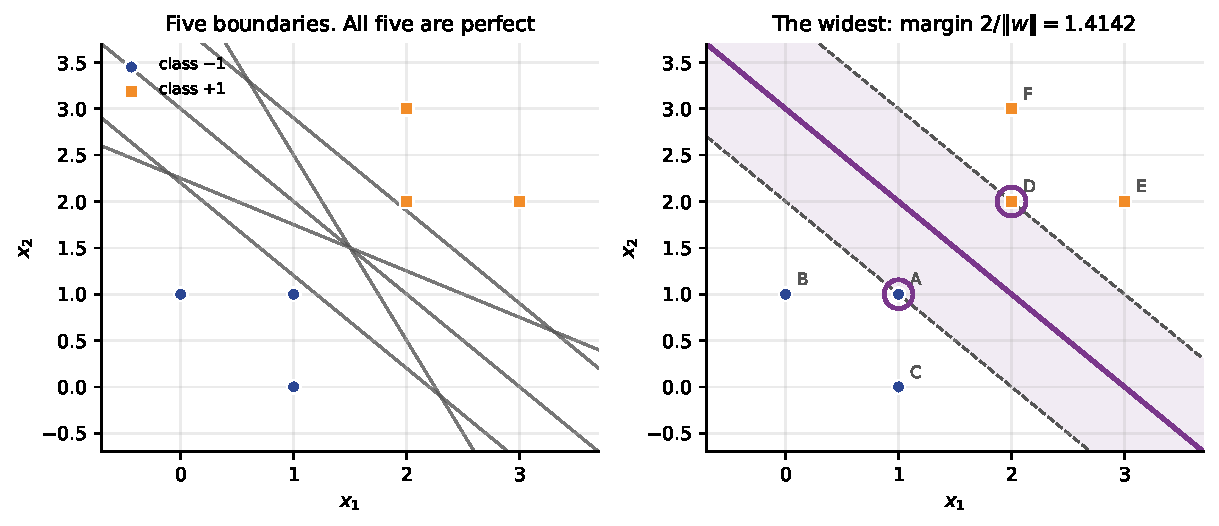
\includegraphics[width=0.72\textwidth]{manylines.pdf}
  \caption{Five lines through the six points. Every one of them classifies all
  six correctly, so every one of them has training accuracy $1.0000$. They are
  visibly not equally good, and the difference has nothing to do with
  accuracy.}
  \label{fig:manylines}
\end{figure}

This is the situation that motivates the entire lecture, so state the problem
precisely: \emph{training accuracy assigns the same score to all of these
lines, and yet they are obviously not equally trustworthy.} A line that skims
past a training point will misclassify a new point drawn from the same place;
a line running down the middle of the empty corridor between the classes has
room to be slightly wrong.

We can measure that difference. For a line $w^\top x + b = 0$, the distance
from a point $x_i$ is $|w^\top x_i + b| / \|w\|$; take the minimum over the
six points and you have a number that says how close the line ever comes to
the data.

\begin{lstlisting}
lines = [(1., 1., -2.2), (1., 1., -3.9), (2., 1., -4.5),
         (1., 2., -4.5), (1., 1., -3.0)]
print("  %-22s %7s %15s %14s"
      % ("line", "errors", "nearest point", "margin width"))
for w1, w2, b in lines:
    w = np.array([w1, w2])
    err = int(np.sum(np.sign(X @ w + b) != y))
    d = np.min(np.abs(X @ w + b) / np.linalg.norm(w))
    print("  %-22s %7d %15.4f %14.4f"
          % ("%gx1 %+gx2 %+g = 0" % (w1, w2, b), err, d, 2 * d))
print("every one of them is a perfect classifier; they are not equally safe")
\end{lstlisting}
\begin{codeout}
  line                    errors   nearest point   margin width
  1x1 +1x2 -2.2 = 0            0          0.1414         0.2828
  1x1 +1x2 -3.9 = 0            0          0.0707         0.1414
  2x1 +1x2 -4.5 = 0            0          0.6708         1.3416
  1x1 +2x2 -4.5 = 0            0          0.6708         1.3416
  1x1 +1x2 -3 = 0              0          0.7071         1.4142
every one of them is a perfect classifier; they are not equally safe
\end{codeout}

Read the second column and then the third. The error count is $0$ five times
over. The clearance ranges from $0.0707$ to $0.7071$ --- a factor of ten. The
last line has ten times the room of the second and scores identically on every
metric computed from predictions alone.

\begin{keyidea}
When several models fit the training data perfectly, accuracy cannot rank
them. The support vector machine ranks them by \textbf{clearance}: how close
the boundary comes to the nearest training point. The whole method is the
consequence of turning that ranking into something a solver can maximise.
\end{keyidea}

\subsection{The distance from a point to a hyperplane}
\label{sec:distance}

In $d$ dimensions the boundary is a \textbf{hyperplane}
$\{x : w^\top x + b = 0\}$ --- a line when $d = 2$, a plane when $d = 3$. Two
facts about it are worth deriving rather than quoting.

First, \textbf{$w$ is perpendicular to the hyperplane}. If $x$ and $x'$ both
lie on it then $w^\top x + b = 0$ and $w^\top x' + b = 0$, so subtracting,
$w^\top(x - x') = 0$. The vector $x - x'$ is an arbitrary direction lying
inside the hyperplane, and $w$ is orthogonal to all of them.

Second, the signed distance. Let $x_p$ be the foot of the perpendicular from
$x$ to the hyperplane, so that $x = x_p + r\,w/\|w\|$ for some scalar $r$ whose
magnitude is the distance and whose sign says which side we are on. Then
\[
  w^\top x + b
  \;=\; \underbrace{w^\top x_p + b}_{=\,0}
        \;+\; r\,\frac{w^\top w}{\|w\|}
  \;=\; r\,\|w\| ,
\]
because $w^\top w = \|w\|^2$. Rearranging,
\begin{equation}
  r \;=\; \frac{w^\top x + b}{\|w\|} .
  \label{eq:signeddist}
\end{equation}

Two different quantities now have to be kept apart, and confusing them is the
commonest source of error in this material.

\begin{itemize}[leftmargin=*]
  \item The \textbf{functional margin} of point $i$ is
    $\hat\gamma_i = y_i\,(w^\top x_i + b)$. It is positive exactly when the
    point is on the correct side, and its size says how confidently.
  \item The \textbf{geometric margin} is
    $\gamma_i = \hat\gamma_i / \|w\| = y_i\,r_i$. It is the actual distance,
    in the units of the feature space, with a sign for correctness.
\end{itemize}

\begin{caution}[The functional margin can be inflated for free]
Replace $(w,b)$ by $(2w,2b)$. The set $\{x : 2w^\top x + 2b = 0\}$ is the
\emph{same set of points} --- the boundary has not moved and no prediction has
changed. But every functional margin has doubled. So the functional margin on
its own is meaningless as an objective: you could maximise it to infinity
without improving the classifier by one row. The geometric margin is
unaffected, because the $\|w\|$ in the denominator doubles too.
\end{caution}

\subsection{Deriving the width: the margin is $2/\|w\|$}
\label{sec:derive}

That redundancy has to be removed before we can optimise anything. The
standard way is to spend it on a convenient normalisation. Since $(w,b)$ and
$(cw, cb)$ describe the same boundary for any $c > 0$, we may choose $c$ so
that
\begin{equation}
  \min_i\; y_i\,(w^\top x_i + b) \;=\; 1 .
  \label{eq:canonical}
\end{equation}
A pair $(w,b)$ satisfying \eqref{eq:canonical} is called the \textbf{canonical}
hyperplane for that dataset. It is not a restriction on which boundaries we may
consider --- every boundary has exactly one canonical representative --- it is
a choice of units.

Now the geometry falls out. Let $x_+$ be a closest point of class $+1$. By
\eqref{eq:canonical} it satisfies $w^\top x_+ + b = +1$, so by
\eqref{eq:signeddist} its distance from the boundary is $1/\|w\|$. Let $x_-$ be
a closest point of class $-1$; it satisfies $w^\top x_- + b = -1$, so it too is
$1/\|w\|$ away, on the other side. Between them lies a slab containing no
training points at all, of width
\begin{equation}
  \text{margin width} \;=\; \frac{1}{\|w\|} + \frac{1}{\|w\|}
  \;=\; \frac{2}{\|w\|} .
  \label{eq:width}
\end{equation}

And therefore --- this is the step the whole method turns on ---
\begin{equation}
  \max_{w,b}\ \frac{2}{\|w\|}
  \iff \min_{w,b}\ \|w\|
  \iff \min_{w,b}\ \tfrac12 \|w\|^2 .
  \label{eq:equiv}
\end{equation}
The first equivalence holds because $t \mapsto 2/t$ is strictly decreasing on
$t > 0$, so whatever maximises $2/\|w\|$ minimises $\|w\|$. The second holds
because $t \mapsto t^2$ is strictly increasing on $t \ge 0$. The $\tfrac12$
and the square are pure convenience: they make the gradient $w$ instead of
$w/\|w\|$, and they change nothing whatever about \emph{where} the minimum is.

\begin{keyidea}[The hard-margin primal]
\[
  \min_{w,\,b}\ \ \tfrac12\|w\|^2
  \qquad\text{subject to}\qquad
  y_i\,(w^\top x_i + b) \;\ge\; 1
  \quad\text{for } i = 1,\dots,n .
\]
A \textbf{convex quadratic objective} under \textbf{linear inequality
constraints}: a convex quadratic program, with one global optimum and no local
minima to get stuck in. Note what is \emph{absent} from the objective --- any
count of how many points are correct. Correctness is in the constraints; the
thing being minimised is purely a measure of how steep the decision function
is.
\end{keyidea}

Each constraint says two things at once. Its sign says the point is on the
right side; its magnitude says the point is at least one functional unit clear
of the boundary. Under the canonical normalisation \eqref{eq:canonical} at
least one constraint holds with equality --- otherwise we could shrink $\|w\|$
further and widen the margin.

\begin{figure}[tb]
  \centering
  
\includegraphics[width=0.56\textwidth]{margin.pdf}
  \caption{The maximum-margin solution for the six points. The solid line is
  $w^\top x + b = 0$ with $w = (1,1)$ and $b = -3$; the dashed lines are
  $w^\top x + b = \pm 1$. Since $\|w\| = \sqrt2$, the empty band between them
  is $2/\|w\| = 1.414214$ wide. Points \textbf{A} and \textbf{D} sit exactly on
  its edges; the other four are strictly outside.}
  \label{fig:margin}
\end{figure}

% =========================================================================
\section{The primal, the Lagrangian and the dual}
\label{sec:dual}

You could stop at the primal and hand it to a general-purpose QP solver, and
for a linear SVM on tabular data that is a perfectly reasonable thing to do.
The reason every treatment of SVMs goes through the dual anyway is not
computational --- it is that the dual makes two things visible that the primal
hides. One is the role of individual training points; the other is the kernel
trick. This section is the price of admission for both.

\subsection{Attaching a multiplier to every constraint}

The method of Lagrange multipliers handles constrained optimisation by folding
each constraint into the objective with a price attached. Write each constraint
in the form $g_i(w,b) = y_i(w^\top x_i + b) - 1 \ge 0$, give it a multiplier
$\alpha_i \ge 0$, and form the \textbf{Lagrangian}
\begin{equation}
  L(w, b, \alpha)
  \;=\; \tfrac12\|w\|^2
        \;-\; \sum_{i=1}^{n} \alpha_i\bigl[\,y_i(w^\top x_i + b) - 1\,\bigr].
  \label{eq:lagrangian}
\end{equation}
The minus sign is the convention for $\ge$ constraints: violating a constraint
makes the bracket negative and so \emph{increases} $L$, which is what a penalty
should do.

At a solution, $L$ is stationary in the primal variables. Differentiating
\eqref{eq:lagrangian} with respect to $w$ --- remembering that
$\partial(\tfrac12 w^\top w)/\partial w = w$ --- and with respect to $b$:
\begin{align}
  \frac{\partial L}{\partial w} = w - \sum_i \alpha_i y_i x_i = 0
  &\quad\Longrightarrow\quad
  \boxed{\; w = \sum_{i=1}^n \alpha_i y_i x_i \;}
  \label{eq:wsum}\\[0.3em]
  \frac{\partial L}{\partial b} = -\sum_i \alpha_i y_i = 0
  &\quad\Longrightarrow\quad
  \boxed{\; \sum_{i=1}^n \alpha_i y_i = 0 \;}
  \label{eq:sumzero}
\end{align}

Read \eqref{eq:wsum} again before going on, because it is a structural fact
about the model and not a step in an algebraic manipulation. \textbf{The weight
vector is a weighted sum of the training points themselves.} The model does not
invent a direction in feature space; it combines the data it was given. And any
training point whose multiplier is zero contributes nothing at all to that sum.

\subsection{Substituting back gives the dual}

Put \eqref{eq:wsum} and \eqref{eq:sumzero} back into \eqref{eq:lagrangian}.
The term in $b$ is $-b\sum_i \alpha_i y_i$, which is zero by
\eqref{eq:sumzero}. The quadratic term becomes
\[
  \tfrac12 \|w\|^2
  = \tfrac12 \sum_i\sum_j \alpha_i\alpha_j y_i y_j \langle x_i, x_j\rangle ,
\]
and the linear term $-\sum_i \alpha_i y_i w^\top x_i$ becomes
$-\sum_i\sum_j \alpha_i\alpha_j y_i y_j \langle x_i, x_j\rangle$, which is
twice the quadratic term with the opposite sign. Adding the leftover
$+\sum_i \alpha_i$ leaves

\begin{keyidea}[The dual problem]
\[
  \max_{\alpha}\ \ \sum_{i=1}^{n}\alpha_i
    \;-\; \tfrac12 \sum_{i=1}^{n}\sum_{j=1}^{n}
      \alpha_i\alpha_j\,y_i y_j\, \langle x_i, x_j\rangle
  \qquad\text{s.t.}\qquad
  \alpha_i \ge 0,\quad \sum_i \alpha_i y_i = 0 .
\]
\end{keyidea}

Two things have happened. The problem is now in $n$ variables (one per training
row) rather than $d + 1$, which is a win whenever $d \gg n$ --- a text
classifier with fifty thousand vocabulary columns and eight hundred documents,
for instance. And, far more importantly:

\begin{keyidea}
The training data appears in the dual \textbf{only} inside the inner products
$\langle x_i, x_j\rangle$. Never as individual coordinates, never in any other
combination. If the algorithm only ever needs inner products, you can change
what ``inner product'' means without changing the algorithm --- and
Section~\ref{sec:kernel} is the whole of what follows from that.
\end{keyidea}

\subsection{The KKT conditions, and the sentence that matters}
\label{sec:kkt}

For a convex problem with linear constraints, the Karush--Kuhn--Tucker
conditions are necessary and sufficient for optimality. Three of them concern
us:
\begin{equation}
  \underbrace{\alpha_i \ge 0}_{\text{dual feasibility}},
  \qquad
  \underbrace{y_i(w^\top x_i + b) - 1 \ge 0}_{\text{primal feasibility}},
  \qquad
  \underbrace{\alpha_i\bigl[\,y_i(w^\top x_i + b) - 1\,\bigr] = 0}
    _{\textbf{complementary slackness}} .
  \label{eq:kkt}
\end{equation}

The third one is doing all the work, and it is doing it in a very simple way:
it says that a product of two numbers is zero, so at least one of them must be.
For every single training point, therefore, one of two things is true:

\begin{itemize}[leftmargin=*]
  \item $\alpha_i = 0$. The point contributes nothing to $w$ in
    \eqref{eq:wsum}. It could be deleted from the training set and the answer
    would be unchanged.
  \item $y_i(w^\top x_i + b) = 1$. The point lies \emph{exactly} on the edge of
    the margin, and it may have $\alpha_i > 0$.
\end{itemize}

\begin{keyidea}[Support vectors]
The training points with $\alpha_i > 0$ are the \textbf{support vectors}. They
lie on the margin, and by \eqref{eq:wsum} the model is a weighted combination
of them alone. Every other row of the training set is a spectator.
\end{keyidea}

That is the definition \emph{earned} rather than announced. Notice that it did
not come from a modelling choice or from an approximation --- it came from a
product being zero at the optimum of a convex program. Section~\ref{sec:sv}
tests it by deleting rows and measuring what moves.

Once $\alpha$ is known, $b$ follows. For any support vector $x_s$ we have
$y_s(w^\top x_s + b) = 1$, and since $y_s \in \{-1, +1\}$ implies
$1/y_s = y_s$, this rearranges to $b = y_s - w^\top x_s$. In practice one
averages over all support vectors for numerical stability:
\begin{equation}
  b \;=\; \frac{1}{|S|}\sum_{s \in S}\bigl(y_s - w^\top x_s\bigr) .
  \label{eq:bias}
\end{equation}

% =========================================================================
\section{Six points, solved completely by hand}
\label{sec:hand}

This is the centrepiece of the lecture. Do not read it passively; do it with a
pen and check your numbers against the printout.

\begin{worked}[The six points of Section~\ref{sec:sixpoints}]
\textbf{Step 1 --- guess the support set.} Support vectors are the points
closest to the opposing class. Looking at the data, the two closest points
across the class boundary are $A = (1,1)$ with $y = -1$ and $D = (2,2)$ with
$y = +1$. Suppose these two are the only ones with $\alpha > 0$. We will
verify the guess afterwards; if it were wrong, some constraint would come out
violated.

\textbf{Step 2 --- use $\sum_i \alpha_i y_i = 0$.} With only $\alpha_A$ and
$\alpha_D$ non-zero, \eqref{eq:sumzero} reads
\[
  (-1)\alpha_A + (+1)\alpha_D = 0
  \quad\Longrightarrow\quad
  \alpha_A = \alpha_D = \alpha .
\]

\textbf{Step 3 --- use $w = \sum_i \alpha_i y_i x_i$.} By \eqref{eq:wsum},
\[
  w = \alpha\bigl[(-1)(1,1) + (+1)(2,2)\bigr]
    = \alpha\bigl[(2,2) - (1,1)\bigr]
    = \alpha\,(1,1) .
\]
So $w$ points along the direction from the negative support vector to the
positive one. That is not a coincidence and it generalises: with one support
vector on each side, $w$ is parallel to $x_+ - x_-$.

\textbf{Step 4 --- both support vectors are on the margin.} Write
$w = (\alpha, \alpha)$ and impose $y_i(w^\top x_i + b) = 1$ for $A$ and $D$:
\[
  \text{$A$:}\quad (-1)\bigl[\alpha\cdot 1 + \alpha\cdot 1 + b\bigr] = 1
  \;\Longrightarrow\; -(2\alpha + b) = 1 ,
\]
\[
  \text{$D$:}\quad (+1)\bigl[\alpha\cdot 2 + \alpha\cdot 2 + b\bigr] = 1
  \;\Longrightarrow\; 4\alpha + b = 1 .
\]
Two linear equations in two unknowns. Adding them eliminates $b$:
\[
  (4\alpha + b) + (-2\alpha - b) = 1 + 1
  \;\Longrightarrow\; 2\alpha = 2
  \;\Longrightarrow\; \boxed{\alpha = 1} .
\]
Substituting back into $4\alpha + b = 1$ gives $b = 1 - 4 = \boxed{-3}$, and
therefore $\boxed{w = (1,1)}$.

\textbf{Step 5 --- verify the guess.} Check the four points we assumed to be
spectators. For $B = (0,1)$: $w^\top x + b = 0 + 1 - 3 = -2$, and
$y\,f = (-1)(-2) = 2 \ge 1$. For $C = (1,0)$: identically $-2$, so
$y\,f = 2$. For $E = (3,2)$: $3 + 2 - 3 = +2$, so $y\,f = 2$. For $F = (2,3)$:
$+2$ again, $y\,f = 2$. Every constraint is satisfied with slack, so
\eqref{eq:kkt} is consistent with $\alpha_B = \alpha_C = \alpha_E =
\alpha_F = 0$. The guess was right.

\textbf{Step 6 --- the margin width.} $\|w\| = \sqrt{1^2 + 1^2} = \sqrt2$, so
\[
  \frac{2}{\|w\|} = \frac{2}{\sqrt 2} = \sqrt 2 = 1.414214 .
\]
\end{worked}

Now the same problem given to the library. Setting $C$ to a very large number
makes the soft margin of Section~\ref{sec:soft} effectively hard, because
violating a constraint becomes prohibitively expensive.

\begin{lstlisting}
w_hand = np.array([1.0, 1.0]); b_hand = -3.0
print("by hand :  w = (%g, %g)   b = %g" % (w_hand[0], w_hand[1], b_hand))
print("           ||w||   = %.10f" % np.linalg.norm(w_hand))
print("           2/||w|| = %.10f" % (2 / np.linalg.norm(w_hand)))
clf = SVC(kernel="linear", C=1e6).fit(X, y)          # C huge = hard margin
print("SVC     :  w =", np.round(clf.coef_[0], 10),
      "  b = %.10f" % clf.intercept_[0])
print("           2/||w|| = %.10f" % (2 / np.linalg.norm(clf.coef_[0])))
print("agree to 1e-9:", bool(np.allclose(clf.coef_[0], w_hand, atol=1e-9)
                             and abs(clf.intercept_[0] - b_hand) < 1e-9))
\end{lstlisting}
\begin{codeout}
by hand :  w = (1, 1)   b = -3
           ||w||   = 1.4142135624
           2/||w|| = 1.4142135624
SVC     :  w = [1. 1.]   b = -3.0000000000
           2/||w|| = 1.4142135624
agree to 1e-9: True
\end{codeout}

Not ``close to''. \textbf{The same numbers.} The library solved, by an
iterative decomposition method on a six-variable quadratic program, exactly the
problem you solved with two linear equations.

\subsection{Reading the functional margins}

The quantity $y_i f(x_i)$ tells you at a glance which points are on the margin.

\begin{lstlisting}
f = X @ clf.coef_[0] + clf.intercept_[0]
print("pt   f(x)     y f(x)   on the margin?")
for n, fi, yi in zip(names, f, y):
    print(" %s  %+6.2f   %+6.2f       %s"
          % (n, fi, yi * fi, "yes" if abs(yi * fi - 1) < TOL else "no"))
\end{lstlisting}
\begin{codeout}
pt   f(x)     y f(x)   on the margin?
 A   -1.00    +1.00       yes
 B   -2.00    +2.00       no
 C   -2.00    +2.00       no
 D   +1.00    +1.00       yes
 E   +2.00    +2.00       no
 F   +2.00    +2.00       no
\end{codeout}

Exactly $1$ on the margin, strictly greater than $1$ outside it. Compare this
column against the $\alpha$ column below and you have complementary slackness
printed twice.

\subsection{The multipliers, and $w$ rebuilt from them}

\texttt{SVC} does not expose $\alpha$ directly. It exposes
\texttt{dual\_coef\_}, which holds the products $\alpha_i y_i$ for the support
vectors only, and \texttt{support\_}, which holds their row indices. Taking
absolute values recovers $\alpha$.

\begin{lstlisting}
alpha = np.zeros(len(X)); alpha[clf.support_] = np.abs(clf.dual_coef_[0])
print("support_        :", clf.support_, "->", " ".join(names[clf.support_]))
print("alpha           :", np.round(alpha, 10))
print("sum_i alpha_i y_i = %.1e   (must be 0)" % float(alpha @ y))
w_dual = (alpha * y) @ X
print("w = sum_i alpha_i y_i x_i =", np.round(w_dual, 10))
b_dual = np.mean(y[clf.support_] - X[clf.support_] @ w_dual)
print("b = mean over SVs of (y_s - w.x_s) = %.10f" % b_dual)
dual_obj = alpha.sum() - 0.5 * w_dual @ w_dual
print("dual objective  = %.10f" % dual_obj)
print("(1/2)||w||^2    = %.10f" % (0.5 * w_dual @ w_dual))
\end{lstlisting}
\begin{codeout}
support_        : [0 3] -> A D
alpha           : [1. 0. 0. 1. 0. 0.]
sum_i alpha_i y_i = 0.0e+00   (must be 0)
w = sum_i alpha_i y_i x_i = [1. 1.]
b = mean over SVs of (y_s - w.x_s) = -3.0000000000
dual objective  = 1.0000000000
(1/2)||w||^2    = 1.0000000000
\end{codeout}

Four of the six multipliers are \textbf{exactly zero}, not small. Equation
\eqref{eq:wsum} reconstructs $w = (1,1)$ from the two that are not, and
\eqref{eq:bias} reconstructs $b = -3$. The constraint \eqref{eq:sumzero} holds
to $0.0\mathrm{e}{+}00$.

The last two lines are worth a sentence. The dual objective at its maximum is
$1.0000000000$; the primal objective $\tfrac12\|w\|^2$ at its minimum is
$1.0000000000$. That equality is what \textbf{strong duality} means: for this
class of problem the two optimisation problems have the same optimal value, so
solving either one solves the other. It is why solvers are free to work on
whichever is more convenient --- and for kernel SVMs the dual is the only one
that can even be written down.

\begin{figure}[tb]
  \centering
  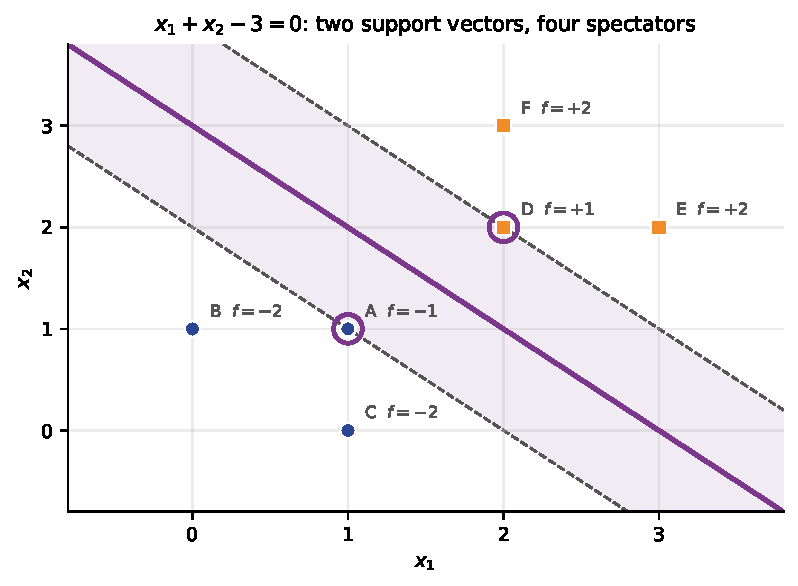
\includegraphics[width=0.60\textwidth]{handsvm.pdf}
  \caption{The solved six-point problem. Circled: the two support vectors, $A$
  and $D$, each with $\alpha = 1$. The line is fixed by exactly two points ---
  the smallest number that can fix a line in the plane, one from each side.}
  \label{fig:handsvm}
\end{figure}

\begin{tryit}[Move a spectator and watch nothing happen]
Change $B$ from $(0,1)$ to $(-5, 4)$ --- a large move, well away from the
boundary --- and refit. You should still get \texttt{w = [1. 1.]},
\texttt{b = -3.0}, and \texttt{support\_ = [0 3]}. Then move $A$ from $(1,1)$
to $(1.2, 1.2)$ and refit: everything changes. One row out of six is doing all
the work.
\end{tryit}

% =========================================================================
\section{Support vectors: the memorable result}
\label{sec:sv}

Section~\ref{sec:kkt} claimed that non-support-vectors could be deleted with no
effect. That is a strong, falsifiable claim, so let us try to falsify it.

\subsection{The deletion experiment}

Refit the six-point problem four times: on all six points, then with $B$
removed (not a support vector), then with $D$ removed (a support vector), then
with $A$ removed (also a support vector).

\begin{lstlisting}
def fit_report(keep, label):
    c = SVC(kernel="linear", C=1e6).fit(X[keep], y[keep])
    w, b = c.coef_[0], c.intercept_[0]
    print("%-26s w = (%.4f, %.4f)  b = %+.4f  nSV = %d  2/||w|| = %.4f"
          % (label, w[0], w[1], b, c.n_support_.sum(),
             2 / np.linalg.norm(w)))
    return w, b

w0, b0 = fit_report(np.arange(6), "all six points")
wB, bB = fit_report([0, 2, 3, 4, 5], "drop B (0,1), not a SV")
fit_report([0, 1, 2, 4, 5], "drop D (2,2), a SV")
fit_report([1, 2, 3, 4, 5], "drop A (1,1), a SV")
print("dropping B moved w by %.2e and b by %.2e -- nothing moved"
      % (np.abs(wB - w0).max(), abs(bB - b0)))
\end{lstlisting}
\begin{codeout}
all six points             w = (1.0000, 1.0000)  b = -3.0000  nSV = 2  2/||w|| = 1.4142
drop B (0,1), not a SV     w = (1.0000, 1.0000)  b = -3.0000  nSV = 2  2/||w|| = 1.4142
drop D (2,2), a SV         w = (0.6665, 0.6670)  b = -2.3337  nSV = 3  2/||w|| = 2.1211
drop A (1,1), a SV         w = (0.6664, 0.6668)  b = -1.6665  nSV = 3  2/||w|| = 2.1215
dropping B moved w by 0.00e+00 and b by 0.00e+00 -- nothing moved
dropping a support vector widened the margin 1.4142 -> 2.1211
\end{codeout}

Be precise about the second row. Dropping $B$ did not produce a small change.
It produced a change of $0.00\mathrm{e}{+}00$ in $w$ and
$0.00\mathrm{e}{+}00$ in $b$, to the printing precision of a float. Most
students, asked to predict this in advance, say ``not much will happen'' and
hedge. The correct answer is that \emph{nothing} happens.

Dropping a support vector, by contrast, moves everything: $w$ falls from
$(1,1)$ to about $(0.667, 0.667)$, $b$ moves, a third point is recruited as a
support vector, and the margin widens by half.

\begin{figure}[tb]
  \centering
  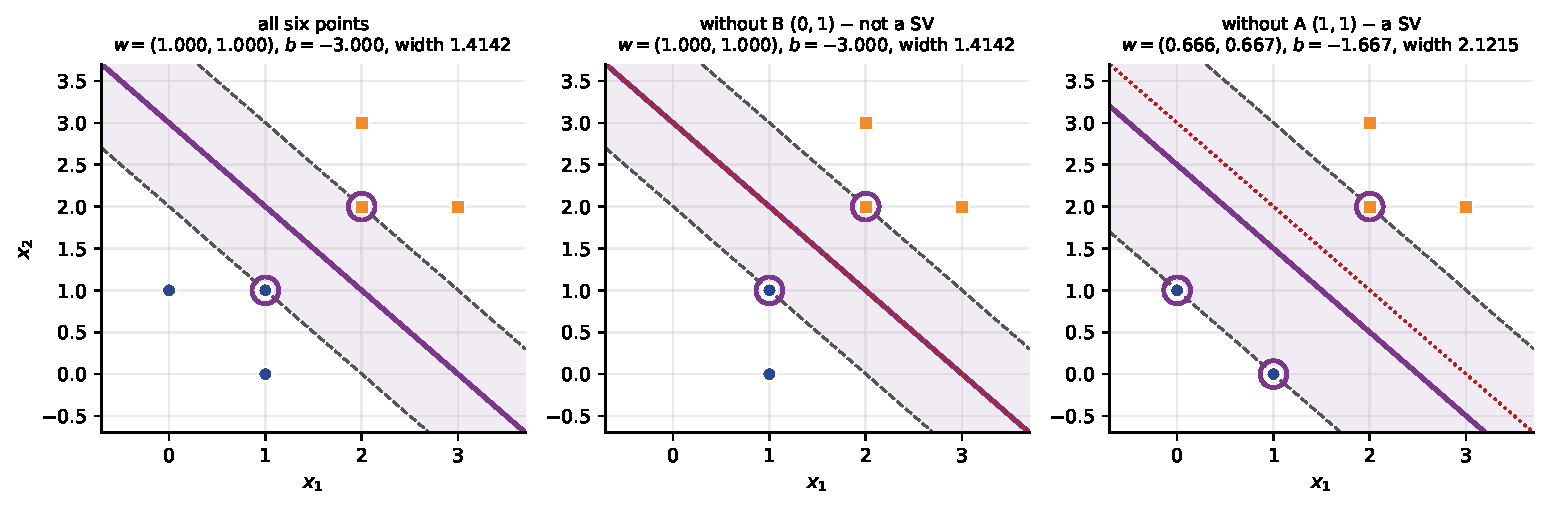
\includegraphics[width=0.94\textwidth]{deletion.pdf}
  \caption{The four fits of the deletion experiment. Left to right: all six
  points; $B$ deleted, which is a spectator and the boundary does not move; $D$
  deleted; $A$ deleted. Removing either support vector removes a constraint and
  the band immediately grows from $1.4142$ to about $2.121$.}
  \label{fig:deletion}
\end{figure}

\subsection{Why the margin got \emph{wider}, and not narrower}

Students often expect deleting a point to make things worse. The primal
explains why the opposite happens. Each training point contributes one
constraint, so deleting a point \emph{removes} a constraint. Minimising
$\tfrac12\|w\|^2$ over a larger feasible set can only give the same value or a
smaller one --- and a smaller $\|w\|$ is a wider band by \eqref{eq:width}.
Deleting a spectator, whose constraint was not active, changes nothing;
deleting a support vector, whose constraint was tight, relaxes the binding
restriction and the margin expands.

\begin{worked}[Check the widened margin by hand]
Delete $A = (1,1)$. The remaining negatives are $B = (0,1)$ and $C = (1,0)$,
and the nearest positive is still $D = (2,2)$. The closest point of the
negative class to $D$ is not $B$ or $C$ individually but a point on the segment
joining them --- the convex hull of $\{B, C\}$ --- and by symmetry that is the
midpoint $(0.5, 0.5)$.

The maximum-margin band is the widest slab separating the two convex hulls, and
its width equals the distance between the closest points of those hulls. Here
that is
\[
  \|(2,2) - (0.5, 0.5)\| = \|(1.5, 1.5)\| = 1.5\sqrt2 = 2.1213 .
\]
The solver reported $2/\|w\| = 2.1215$. The two agree to four significant
figures; the discrepancy in the fourth decimal is the $10^{-3}$ stopping
tolerance, not a different answer.
\end{worked}

\begin{keyidea}[The examinable sentence]
\textbf{The support vectors \emph{are} the training set.} Delete every other
row and you obtain the identical model. Delete one support vector and the
boundary moves. That is what $\alpha_i = 0$ \emph{means} --- not ``this point
matters a little'', but ``this point does not enter the model at all''.
\end{keyidea}

\subsection{Not a toy effect: throw away $69$ of $80$ rows}

Six points is a demonstration. Here is the same property on a real fit, on
eighty points from \texttt{make\_blobs} with substantial overlap and an
ordinary $C = 1$.

\begin{lstlisting}
Xb, yb = make_blobs(n_samples=80, centers=2, cluster_std=2.4, random_state=3)
yb = np.where(yb == 0, -1, 1)
full = SVC(kernel="linear", C=1.0).fit(Xb, yb)             # 80 points
sv = full.support_
only = SVC(kernel="linear", C=1.0).fit(Xb[sv], yb[sv])     # 11 points
print("trained on all %d points : w = %s  b = %+.6f"
      % (len(yb), np.round(full.coef_[0], 6), full.intercept_[0]))
print("trained on the %d SVs only: w = %s  b = %+.6f"
      % (len(sv), np.round(only.coef_[0], 6), only.intercept_[0]))
print("identical predictions on all 80 points:",
      bool(np.all(full.predict(Xb) == only.predict(Xb))))
print("the other %d rows changed nothing" % (len(yb) - len(sv)))
\end{lstlisting}
\begin{codeout}
trained on all 80 points : w = [-0.976353 -0.408819]  b = -1.475724
trained on the 11 SVs only: w = [-0.975901 -0.40859 ]  b = -1.475336
identical predictions on all 80 points: True
the other 69 rows changed nothing
\end{codeout}

Eighty-six per cent of the training set could be deleted \emph{after the fit}
with no change to a single prediction. The coefficients differ in the fourth
decimal place because the solver stops at its tolerance from a different
starting point, not because the answer is different.

\begin{caution}[The same property is the SVM's weakness]
If the model is determined by a handful of rows near the boundary, then a
single mislabelled or anomalous row that happens to land near the boundary
becomes a support vector and drags the whole model with it. A random forest
averages such a row away; an SVM promotes it to a decision-maker. The soft
margin of Section~\ref{sec:soft} exists partly to blunt this, by capping how
much influence any one point may have.
\end{caution}

% =========================================================================
\section{The soft margin and $C$}
\label{sec:soft}

\subsection{Hard margin fails on real data, and it fails completely}

Real data is not separable. Two patients with nearly identical measurements
receive different diagnoses; two customers with the same profile behave
differently. If no hyperplane separates the classes then there is no $(w,b)$
satisfying every constraint $y_i(w^\top x_i + b) \ge 1$, the feasible set of
the primal is \emph{empty}, and the solver does not return a poor answer ---
there is no answer to return.

The fix is to allow constraints to be broken, and to charge for it. Give each
point a \textbf{slack variable} $\xi_i \ge 0$ and weaken its constraint to
\[
  y_i(w^\top x_i + b) \;\ge\; 1 - \xi_i ,
\]
then put the total slack into the objective.

\begin{keyidea}[The soft-margin primal]
\[
  \min_{w,\,b,\,\xi}\ \ \tfrac12\|w\|^2 \;+\; C\sum_{i=1}^{n}\xi_i
  \qquad\text{s.t.}\qquad
  y_i(w^\top x_i + b) \ge 1 - \xi_i,\quad \xi_i \ge 0 .
\]
\end{keyidea}

The constant $C > 0$ is the exchange rate between the two things we want: a
wide margin (small $\|w\|^2$) and few violations (small $\sum \xi_i$). It is
the only new hyperparameter, and it is the one everyone gets backwards.

\subsection{What $\xi_i$ measures, in three regimes}

At the optimum each $\xi_i$ is as small as its constraint allows, which means
$\xi_i = \max(0,\, 1 - y_i f(x_i))$. Three cases:

\begin{itemize}[leftmargin=*]
  \item $\xi_i = 0$: the point is outside the margin on the correct side. It
    has paid nothing. On a well-behaved dataset most points are here.
  \item $0 < \xi_i \le 1$: the point is inside the margin band but still on the
    correct side of the boundary. It is classified correctly and it still
    costs, because it is intruding on the clearance we were trying to buy.
  \item $\xi_i > 1$: the point is past the boundary --- \textbf{misclassified}.
    The number of points with $\xi_i > 1$ is the training error count.
\end{itemize}

The dual changes by exactly one thing. Carrying the $\xi_i$ through the
Lagrangian introduces a second family of multipliers for the constraints
$\xi_i \ge 0$, and eliminating them yields the same dual objective as before
under
\begin{equation}
  0 \;\le\; \alpha_i \;\le\; C ,
  \qquad \sum_i \alpha_i y_i = 0 .
  \label{eq:boxconstraint}
\end{equation}
That box constraint --- an upper limit on how large any single multiplier may
become --- is \textbf{the entire mathematical content of the soft margin}. It
also makes the ``one outlier drags the model'' problem quantitative: no point
can pull with force greater than $C$.

\subsection{$C$ trades margin width against violations, measured}

Fit the eighty-point overlapping problem at five values of $C$ and count
everything.

\begin{lstlisting}
print("     C   nSV   2/||w||   sum of slacks   inside margin   wrong side   train acc")
for C in [0.01, 0.1, 1.0, 10.0, 1000.0]:
    c = SVC(kernel="linear", C=C).fit(Xb, yb)
    m = yb * c.decision_function(Xb)
    slack = np.maximum(0.0, 1 - m)
    print("%6g   %3d    %6.4f        %8.4f              %3d          %3d      %.4f"
          % (C, c.n_support_.sum(), 2 / np.linalg.norm(c.coef_[0]),
             slack.sum(), int(np.sum(m < 1 - TOL)), int(np.sum(m < 0)),
             c.score(Xb, yb)))
\end{lstlisting}
\begin{codeout}
     C   nSV   2/||w||   sum of slacks   inside margin   wrong side   train acc
  0.01    35    5.2135         17.8304               32            3      0.9625
   0.1    18    2.1750          8.3313               15            3      0.9625
     1    11    1.8895          7.6247                8            3      0.9625
    10     9    1.5278          7.5279                6            3      0.9625
  1000     8    1.3483          7.5128                5            3      0.9625
small C buys a wide margin by letting 32 points sit inside it;
large C shrinks the margin until only 5 are left in violation
\end{codeout}

Read the second and fifth columns together. At $C = 0.01$ the model buys a band
$5.2135$ wide and pays for it by letting $32$ of $80$ points sit inside it. At
$C = 1000$ the band is squeezed to $1.3483$ and only $5$ points remain inside.
The support-vector count tracks the same thing, falling from $35$ to $8$,
because under the soft margin every point with $\xi_i > 0$ is also a support
vector.

\begin{caution}[Report the column that does not move]
\textbf{Training accuracy is $0.9625$ in every row}, and the same three points
are misclassified throughout. On this dataset $C$ changes the geometry
enormously and the training score not at all. That is not a curiosity, it is
the reason you cannot tune $C$ on the training set: the quantity you would be
optimising is constant.
\end{caution}

\begin{figure}[tb]
  \centering
  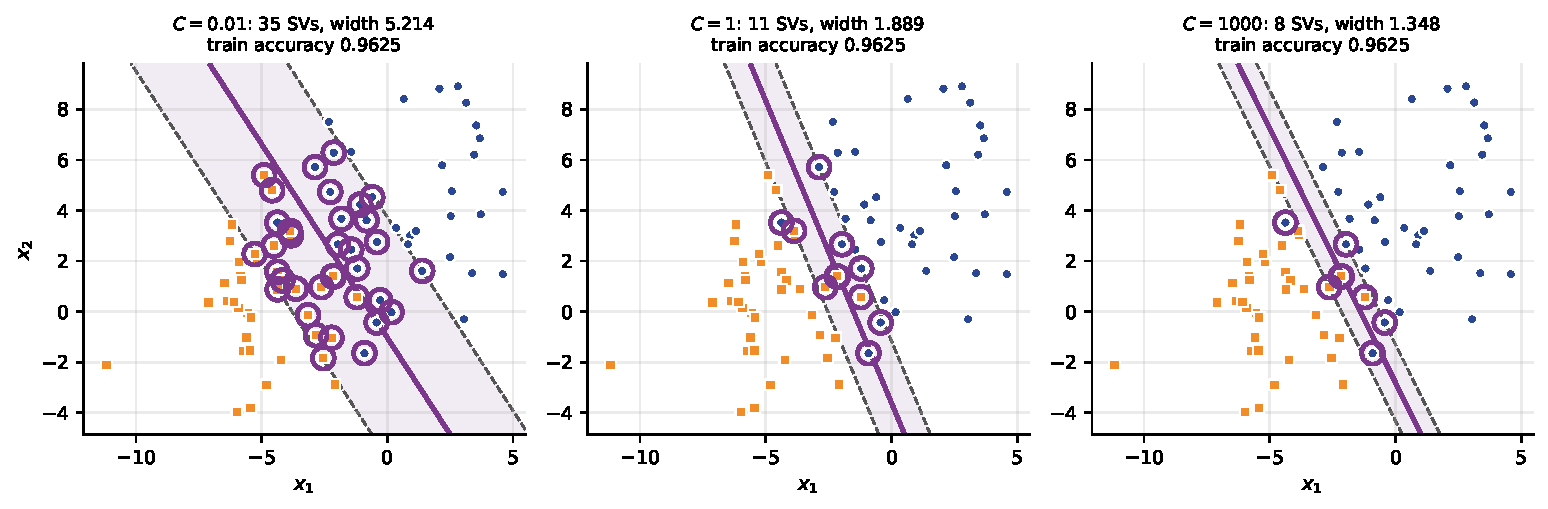
\includegraphics[width=0.94\textwidth]{softc.pdf}
  \caption{The same eighty points at $C = 0.01$, $1$ and $1000$. The shaded
  band is the margin; the ringed points are the support vectors. Small $C$
  means a \emph{soft}, tolerant, well-populated margin; large $C$ means a
  narrow one defended by a few points.}
  \label{fig:softc}
\end{figure}

\subsection{Strong duality again, and three kinds of $\alpha$}

The box constraint \eqref{eq:boxconstraint} sorts the training points into
three classes, and it is worth counting them.

\begin{lstlisting}
C = 1.0
c = SVC(kernel="linear", C=C).fit(Xb, yb)
w, b = c.coef_[0], c.intercept_[0]
m = yb * (Xb @ w + b)
primal = 0.5 * w @ w + C * np.maximum(0.0, 1 - m).sum()
a = np.zeros(len(yb)); a[c.support_] = np.abs(c.dual_coef_[0])
K = Xb @ Xb.T
dual = a.sum() - 0.5 * (a * yb) @ K @ (a * yb)
print("primal  (1/2)||w||^2 + C*sum(hinge) = %.6f" % primal)
print("dual    sum(a) - 1/2 sum a_i a_j y_i y_j x_i.x_j = %.6f" % dual)
print("gap                                  = %.2e" % abs(primal - dual))
print("0 < alpha < C  (on the margin)  : %d points"
      % int(np.sum((a > TOL) & (a < C - TOL))))
print("alpha = C      (inside or wrong): %d points" % int(np.sum(a >= C - TOL)))
print("alpha = 0      (spectators)     : %d points" % int(np.sum(a <= TOL)))
\end{lstlisting}
\begin{codeout}
primal  (1/2)||w||^2 + C*sum(hinge) = 8.184919
dual    sum(a) - 1/2 sum a_i a_j y_i y_j x_i.x_j = 8.184597
gap                                  = 3.22e-04
0 < alpha < C  (on the margin)  : 3 points
alpha = C      (inside or wrong): 8 points
alpha = 0      (spectators)     : 69 points
\end{codeout}

The gap of $3.22\times10^{-4}$ is not a duality gap. For a convex quadratic
program strong duality holds and the true gap is exactly zero; what we are
seeing is \texttt{libsvm} stopping when the KKT conditions hold to $10^{-3}$.
The three counts add to $80$, and the $11$ support vectors of the previous
section are now identified precisely: $3$ sitting on the margin with
$0 < \alpha < C$, and $8$ pinned at the ceiling $\alpha = C$ because they are
inside the band or on the wrong side.

\subsection{$C$ is inverse regularisation}
\label{sec:invreg}

Here is the sweep that settles the question. \texttt{breast\_cancer}, scaled,
linear kernel, and for each $C$ we record the norm of the weight vector, the
five-fold cross-validated accuracy and the support-vector count.

\begin{lstlisting}
print("      C      ||w||    5-fold CV   nSV")
for Cv in [0.001, 0.01, 0.1, 1.0, 10.0, 100.0]:
    p = make_pipeline(StandardScaler(), SVC(kernel="linear", C=Cv)).fit(Xc, yc)
    cv = cross_val_score(make_pipeline(StandardScaler(),
                                       SVC(kernel="linear", C=Cv)),
                         Xc, yc, cv=CV).mean()
    print("%7g   %8.4f   %.4f      %d"
          % (Cv, np.linalg.norm(p[-1].coef_[0]), cv, p[-1].n_support_.sum()))
print("large C -> large ||w|| -> narrow margin -> LESS regularisation")
\end{lstlisting}
\begin{codeout}
      C      ||w||    5-fold CV   nSV
  0.001     0.3555   0.9385      252
   0.01     0.7265   0.9701      118
    0.1     1.4800   0.9772      60
      1     3.0669   0.9754      40
     10     7.9741   0.9631      37
    100    20.8998   0.9613      31
large C -> large ||w|| -> narrow margin -> LESS regularisation
\end{codeout}

As $C$ climbs from $0.001$ to $100$, $\|w\|$ climbs from $0.3555$ to
$20.8998$ --- a factor of nearly sixty. By \eqref{eq:width} the margin shrinks
by the same factor. A model with a large $\|w\|$ has a steep decision function
that swings hard over a short distance: a \emph{complex} model.

\begin{keyidea}[$C$ is inverse regularisation]
Divide the soft-margin objective by $C$:
\[
  \tfrac12\|w\|^2 + C\sum_i \xi_i
  \qquad\longrightarrow\qquad
  \frac{1}{2C}\|w\|^2 + \sum_i \xi_i .
\]
Dividing by a positive constant does not move the minimiser. In this form the
penalty on $\|w\|^2$ is $1/(2C)$, so it is $\lambda = 1/C$ that plays the role
that $\lambda$ plays in ridge regression. \textbf{Large $C$ means small
$\lambda$ means \emph{less} regularisation.}
\end{keyidea}

\begin{caution}[The habit to unlearn]
``A large $C$ regularises more'' is the single most common wrong sentence in
this topic, and it is wrong in a way that costs marks and misconfigures grid
searches. The mnemonic that works: \textbf{big $C$ = big Cost of an error = the
model tries hard to fit every point = complex model}. If you can only remember
one thing from this section, remember $\lambda = 1/C$.
\end{caution}

Note also that this is a genuine tuning parameter and not a knob to turn to an
extreme. The best cross-validated score in the table is $\mathbf{0.9772}$ at
$C = 0.1$, and \emph{both} ends of the sweep are worse --- $0.9385$ at
$C = 0.001$ and $0.9613$ at $C = 100$.

\begin{figure}[tb]
  \centering
  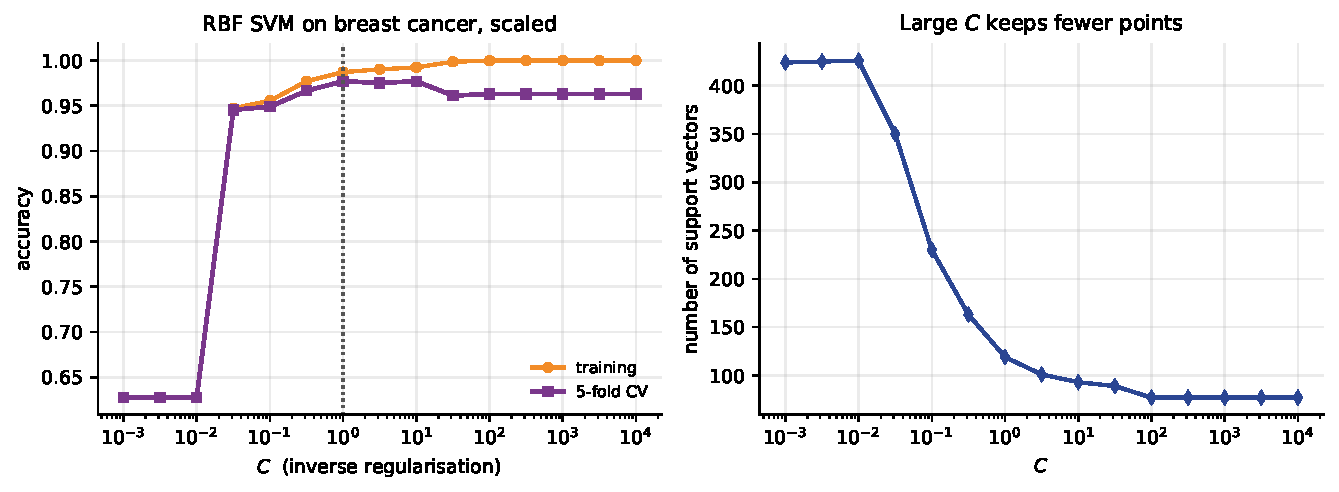
\includegraphics[width=0.94\textwidth]{cvalid.pdf}
  \caption{Left: training and five-fold cross-validated accuracy for an RBF
  SVM on scaled \texttt{breast\_cancer} across fifteen values of $C$. Training
  accuracy climbs monotonically to $1.0000$ and stays; cross-validated accuracy
  peaks at $0.9771$ and then falls to $0.9631$. Right: the support-vector count
  over the same sweep, dropping from $426$ to $77$. \textbf{The gap between the
  two curves in the left panel is the diagnostic}, not either curve alone.}
  \label{fig:cvalid}
\end{figure}

% =========================================================================
\section{The loss the SVM minimises}
\label{sec:hinge}

\subsection{Eliminating the slack variables}

The soft-margin primal has $n$ extra variables in it, one per training point,
and they are not really free: at the optimum each $\xi_i$ takes the smallest
value its two constraints permit,
\[
  \xi_i = \max\bigl(0,\; 1 - y_i f(x_i)\bigr),
  \qquad f(x) = w^\top x + b .
\]
Substituting that back removes the constraints entirely and leaves an
unconstrained problem:
\begin{equation}
  \min_{w,\,b}\ \
  \underbrace{\sum_{i=1}^{n}\max\bigl(0,\ 1 - y_i f(x_i)\bigr)}
    _{\textbf{hinge loss}}
  \;+\; \frac{1}{2C}\,\|w\|^2 .
  \label{eq:hingeobj}
\end{equation}

You have met the function $\max(0, 1 - m)$ before. It appeared in the
loss-functions lecture of Unit II, alongside squared error, absolute error and
the cross-entropies, as one curve among several --- the one that is a straight
ramp down to $m = 1$ and then flat zero forever after. At the time it was
introduced as ``the SVM loss'' without a model attached to it.

\begin{keyidea}
\textbf{The SVM is the model whose loss is the hinge.} Equation
\eqref{eq:hingeobj} is a loss plus an $L_2$ penalty, exactly like ridge
regression or $L_2$-penalised logistic regression; the only thing that
distinguishes an SVM from those is which loss sits in the first term.
\end{keyidea}

\subsection{Why the flat part is the whole story}

Look at where the hinge is exactly zero: for every $m = y_i f(x_i) > 1$. A
point comfortably outside the margin contributes \emph{no loss and no
gradient}. Nudging $w$ slightly does not change its contribution, because its
contribution is identically zero over a whole region, not merely small. That is
precisely the analytic shadow of $\alpha_i = 0$: the point is not participating.

Compare logistic loss, $\log(1 + e^{-m})$, which is positive for every finite
$m$. It decays exponentially, but it never reaches zero, so \emph{every}
training row contributes a gradient at every step, forever. That single
difference --- flat versus asymptotic --- is the difference between a sparse
model and a dense one.

\begin{figure}[tb]
  \centering
  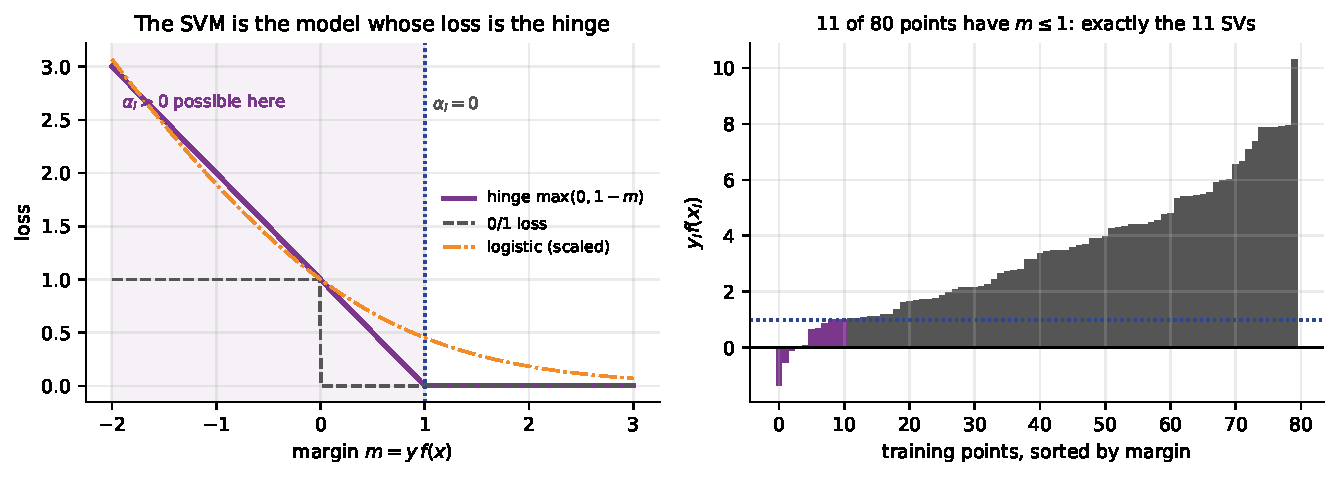
\includegraphics[width=0.94\textwidth]{hinge.pdf}
  \caption{Left: the hinge $\max(0, 1-m)$ against the margin $m = y f(x)$,
  with logistic and $0/1$ loss for comparison. The hinge is exactly zero for
  $m > 1$. Right: the distribution of $m$ over the eighty-point problem;
  $\mathbf{11}$ of $80$ points have $m \le 1$, and \texttt{n\_support\_} is
  $\mathbf{11}$. The same eleven points.}
  \label{fig:hinge}
\end{figure}

\subsection{Same loss, two different solvers}

If \eqref{eq:hingeobj} really is the SVM's objective, then any solver that
minimises it should land in the same place. Two do: \texttt{LinearSVC} with
\texttt{loss='hinge'}, which uses a dedicated coordinate-descent routine, and
\texttt{SGDClassifier} with \texttt{loss='hinge'}, which does plain stochastic
gradient descent. The regularisation parameters have to be matched:
\texttt{SGDClassifier} uses $\alpha$ per-sample where \texttt{LinearSVC} uses
$C$ on the sum, so $\alpha = 1/(Cn)$.

\begin{lstlisting}
Xs = StandardScaler().fit_transform(Xc)
lsvc = LinearSVC(C=0.01, loss="hinge", max_iter=200000).fit(Xs, yc)
sgd = SGDClassifier(loss="hinge", alpha=1.0 / (0.01 * len(yc)),
                    max_iter=20000, tol=1e-6, random_state=0).fit(Xs, yc)
ys = np.where(yc == 1, 1, -1)

def objective(w, b, C):
    m = ys * (Xs @ w + b)
    return 0.5 * w @ w + C * np.maximum(0.0, 1 - m).sum()
\end{lstlisting}
\begin{codeout}
LinearSVC(loss='hinge', C=0.01)
   ||w|| = 0.7599   mean hinge = 0.104136   objective = 0.8812   acc = 0.9842
SGDClassifier(loss='hinge', matched alpha)
   ||w|| = 0.7389   mean hinge = 0.105196   objective = 0.8716   acc = 0.9719
same loss, same regulariser, two different solvers
\end{codeout}

Two entirely different algorithms, two nearly identical norms
($0.7599$ against $0.7389$) and two nearly identical mean hinge losses
($0.104136$ against $0.105196$). They are solving the same problem.

\subsection{Hinge against logistic, on the same data}

\begin{lstlisting}
sv_lin = SVC(kernel="linear", C=1.0).fit(Xs, yc)
lr = LogisticRegression(C=1.0, max_iter=5000).fit(Xs, yc)
\end{lstlisting}
\begin{codeout}
SVC(linear)          uses 40 of 569 rows (the support vectors)
LogisticRegression   uses 569 of 569 rows (every one has a gradient)
cosine between the two weight vectors = 0.9132
5-fold CV  SVC 0.9754   LogisticRegression 0.9789
\end{codeout}

The SVM's model is built from $40$ rows; the logistic model's from all $569$.
And yet the two weight vectors point almost the same way --- cosine $0.9132$ ---
and the cross-validated scores are within $0.0035$ of each other, with logistic
regression marginally ahead. \textbf{Different loss, similar answer, very
different internals.} The practical consequences are real, though: the SVM
gives you a compact model and no probabilities; logistic regression gives you
calibrated probabilities and a model that references every row.

% =========================================================================
\section{The kernel trick}
\label{sec:kernel}

\subsection{A problem no line can solve}

\texttt{make\_circles} produces two concentric groups: an inner blob and an
outer ring. The class is determined entirely by the distance from the origin.
No straight line in the plane can express ``inside a circle'', and a linear
SVM is correspondingly helpless.

\begin{lstlisting}
Xr, yr = make_circles(n_samples=220, factor=0.42, noise=0.09, random_state=0)
yr = np.where(yr == 0, 1, -1)
lin = SVC(kernel="linear", C=1.0).fit(Xr, yr)
Z3 = np.c_[Xr, Xr[:, 0] ** 2 + Xr[:, 1] ** 2]          # add one column
lift = SVC(kernel="linear", C=10.0).fit(Z3, yr)
pol = SVC(kernel="poly", degree=2, gamma=1.0, coef0=1.0, C=1.0).fit(Xr, yr)
\end{lstlisting}
\begin{codeout}
linear SVM, raw (x1,x2)             accuracy 0.5682
linear SVM, (x1,x2,x1^2+x2^2)       accuracy 1.0000
degree-2 polynomial kernel, raw     accuracy 1.0000
the lifted plane: w = [ 0.2076 -0.0436  6.3956]  b = -3.4436
\end{codeout}

A linear SVM scores $\mathbf{0.5682}$ on \emph{its own training data}. That is
barely above the majority class. It is not badly tuned and no amount of tuning
would help; the model class simply cannot express the boundary.

Add one column, $z = x_1^2 + x_2^2$, and the same linear SVM scores
$\mathbf{1.0000}$. In the three-dimensional space $(x_1, x_2, z)$ the inner
blob sits low and the outer ring sits high, so a flat plane $z = c$ separates
them; projected back down to two dimensions, that plane is a circle. Linear
model, curved boundary.

Look at the weight vector of the lifted model: $0.2076$ and $-0.0436$ on the
two original coordinates, and $6.3956$ on the radius column. The model has
discovered on its own that only the third feature matters.

\begin{figure}[tb]
  \centering
  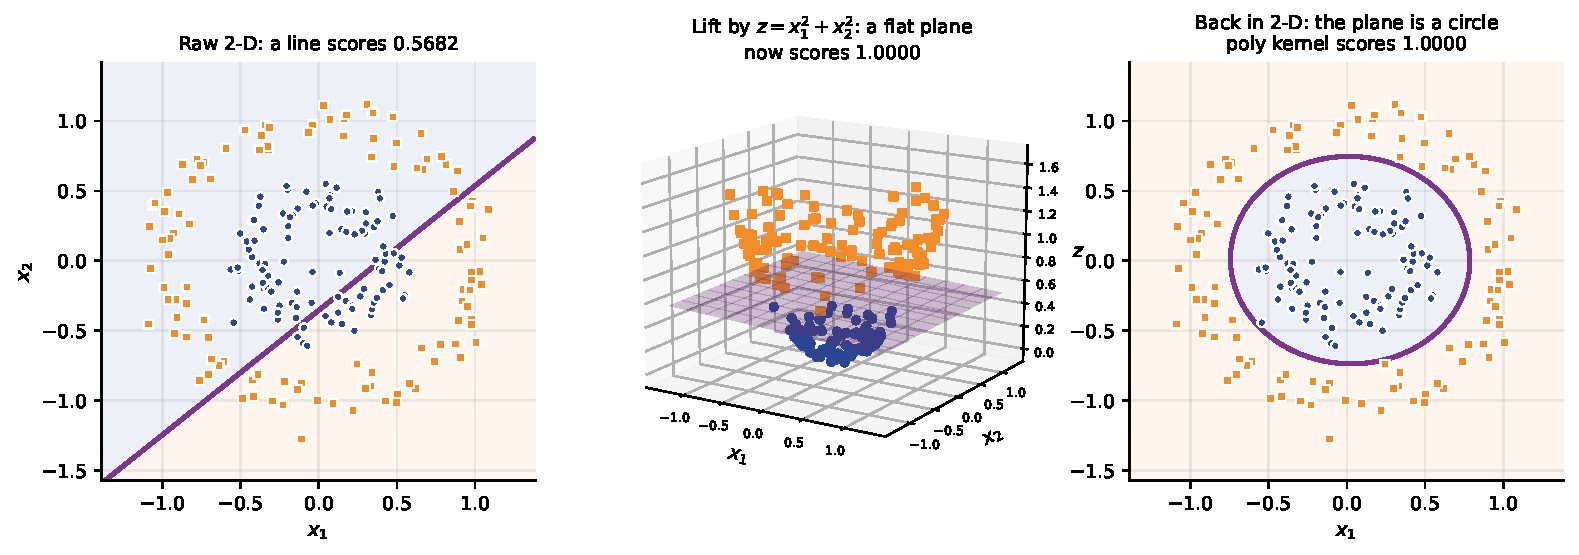
\includegraphics[width=0.98\textwidth]{kernelmap.pdf}
  \caption{Left: the concentric-circles data, which no line separates. Middle:
  the same points lifted to $(x_1, x_2, x_1^2 + x_2^2)$, where a flat plane
  does separate them. Right: that plane brought back down to the plane, where
  it is a circle. Accuracy $0.5682 \to 1.0000$ from one extra column.}
  \label{fig:kernelmap}
\end{figure}

\subsection{The trick: never build the new columns}
\label{sec:kernelid}

Adding a column by hand worked because we happened to know the right column to
add. In general we do not, so the honest version of the strategy is: add
\emph{all} the columns of some degree, and let the optimiser pick. For two
input features and degree two, ``all the columns'' means the map
\begin{equation}
  \varphi(x) = \bigl(1,\ \sqrt2\,x_1,\ \sqrt2\,x_2,\
                  x_1^2,\ x_2^2,\ \sqrt2\,x_1x_2\bigr) \in \mathbb{R}^6 .
  \label{eq:phi2}
\end{equation}
Two features become six. In thirty dimensions at degree three it is $5456$; we
will count these properly in a moment.

Now recall the one structural fact from Section~\ref{sec:dual}: the dual needs
the data only as inner products. So what the algorithm actually requires is
$\langle \varphi(x_i), \varphi(x_j)\rangle$, never $\varphi(x_i)$ itself. And
those inner products have a closed form:
\begin{equation}
  \langle \varphi(x), \varphi(z)\rangle
  \;=\; \bigl(1 + \langle x, z\rangle\bigr)^2 .
  \label{eq:polyid}
\end{equation}

The left-hand side means: build two six-vectors, then take a six-dimensional
dot product. The right-hand side means: take a \emph{two}-dimensional dot
product, add one, square. Same number, and the six-dimensional space is never
constructed.

That is a claim, and claims get checked.

\begin{worked}[Verify \eqref{eq:polyid} at $x = (1,2)$, $z = (3,1)$]
\textbf{Right-hand side, with a pen.}
\[
  \langle x, z\rangle = 1\cdot3 + 2\cdot1 = 5,
  \qquad (1 + 5)^2 = 36 .
\]

\textbf{Left-hand side, term by term.} From \eqref{eq:phi2},
\[
  \varphi(x) = \bigl(1,\ \sqrt2,\ 2\sqrt2,\ 1,\ 4,\ 2\sqrt2\bigr),
  \qquad
  \varphi(z) = \bigl(1,\ 3\sqrt2,\ \sqrt2,\ 9,\ 1,\ 3\sqrt2\bigr).
\]
Multiply componentwise and add:
\[
  \underbrace{1\cdot1}_{1}
  + \underbrace{\sqrt2\cdot3\sqrt2}_{6}
  + \underbrace{2\sqrt2\cdot\sqrt2}_{4}
  + \underbrace{1\cdot9}_{9}
  + \underbrace{4\cdot1}_{4}
  + \underbrace{2\sqrt2\cdot3\sqrt2}_{12}
  \;=\; 1 + 6 + 4 + 9 + 4 + 12 \;=\; 36 .
\]
\textbf{The same number.} Not approximately: the $\sqrt2$ factors in
\eqref{eq:phi2} exist precisely so that the cross terms come out with the
binomial coefficients that $(1 + \langle x,z\rangle)^2$ generates.
\end{worked}

And in code, to ten decimal places:

\begin{lstlisting}
r2 = np.sqrt(2.0)
def phi2(v):
    x1, x2 = v
    return np.array([1.0, r2*x1, r2*x2, x1*x1, x2*x2, r2*x1*x2])

xa = np.array([1.0, 2.0]); za = np.array([3.0, 1.0])
print("x =", xa, "  z =", za)
print("x.z            = %.10f" % (xa @ za))
print("(1 + x.z)^2    = %.10f" % (1 + xa @ za) ** 2)
print("phi(x) =", np.round(phi2(xa), 6))
print("phi(z) =", np.round(phi2(za), 6))
print("phi(x).phi(z)  = %.10f" % (phi2(xa) @ phi2(za)))
print("difference     = %.2e" % abs((1 + xa @ za) ** 2 - phi2(xa) @ phi2(za)))
\end{lstlisting}
\begin{codeout}
x = [1. 2.]   z = [3. 1.]
x.z            = 5.0000000000
(1 + x.z)^2    = 36.0000000000
phi(x) = [1.       1.414214 2.828427 1.       4.       2.828427]
phi(z) = [1.       4.242641 1.414214 9.       1.       4.242641]
phi(x).phi(z)  = 36.0000000000
difference     = 0.00e+00
2 features -> 6, and the kernel never built either vector
\end{codeout}

\begin{keyidea}[The kernel trick]
A \textbf{kernel} is a function $K(x,z)$ that equals
$\langle \varphi(x), \varphi(z)\rangle$ for some feature map $\varphi$.
Replace every $\langle x_i, x_j\rangle$ in the dual with $K(x_i, x_j)$ and you
have trained a linear SVM in the space that $\varphi$ maps into ---
\textbf{without ever writing down a single vector in that space}. The decision
function follows the same route:
\[
  f(x) = \sum_{i \in \mathrm{SV}} \alpha_i y_i\,K(x_i, x) + b .
\]
\end{keyidea}

\subsection{One lucky pair is not evidence}

Two vectors could agree by accident. Check the identity over a whole Gram
matrix, and against scikit-learn's own implementation.

\begin{lstlisting}
rng = np.random.default_rng(0)
V = rng.normal(size=(200, 2))
Kk  = (1 + V @ V.T) ** 2                       # the kernel, 2-D arithmetic
Phi = np.array([phi2(v) for v in V])           # the explicit 6-D map
Ke  = Phi @ Phi.T                              # its Gram matrix
Ks  = polynomial_kernel(V, V, degree=2, gamma=1.0, coef0=1.0)
\end{lstlisting}
\begin{codeout}
kernel matrix       : 200 x 200
explicit map        : 200 x 6, then a 200 x 200 Gram matrix
max |K - phi phi^T| = 2.842e-14
max |K - sklearn|   = 0.000e+00
multiplications, explicit map: 240000
multiplications, kernel      : 80000
\end{codeout}

Forty thousand entries, and the worst disagreement anywhere is
$2.8\times10^{-14}$ --- floating-point rounding, not mathematics. Against
scikit-learn's \texttt{polynomial\_kernel} the difference is exactly $0$.

\subsection{The map you did not have to build}

The saving in the last line above --- $240\,000$ multiplications against
$80\,000$ --- looks like a factor of three, which would hardly justify a
famous name. The point is what happens as the dimension and the degree grow.
The explicit map for degree $p$ in $d$ dimensions has $\binom{d+p}{p}$
features.

\begin{lstlisting}
from math import comb
for d in [2, 10, 30, 100]:
    for deg in [2, 3, 5]:
        print("d = %3d, degree %d -> explicit map has %8d features"
              % (d, deg, comb(d + deg, deg)))
\end{lstlisting}
\begin{codeout}
d =   2, degree 2 -> explicit map has        6 features
d =   2, degree 3 -> explicit map has       10 features
d =   2, degree 5 -> explicit map has       21 features
d =  10, degree 2 -> explicit map has       66 features
d =  10, degree 3 -> explicit map has      286 features
d =  10, degree 5 -> explicit map has     3003 features
d =  30, degree 2 -> explicit map has      496 features
d =  30, degree 3 -> explicit map has     5456 features
d =  30, degree 5 -> explicit map has   324632 features
d = 100, degree 2 -> explicit map has     5151 features
d = 100, degree 3 -> explicit map has   176851 features
d = 100, degree 5 -> explicit map has 96560646 features
the kernel evaluates every one of them with d + 1 multiplications
\end{codeout}

At $d = 100$ and degree $5$ the explicit map has \textbf{ninety-six million}
columns. Storing one such vector in double precision takes about
$772$ megabytes; storing a design matrix of them for even a thousand rows is
out of the question. Meanwhile $(1 + x^\top z)^5$ costs a hundred
multiplications for the dot product, one addition and one power. This is not an
optimisation. It is the difference between possible and impossible.

\subsection{The kernel machine \emph{is} the explicit-map machine}

One more check, because it closes the argument. Fit a degree-2 polynomial
kernel SVM on the circles data, and separately fit a \emph{linear} SVM on the
explicitly constructed $\varphi$-features. If the trick is real, these are the
same model.

\begin{lstlisting}
Pk = SVC(kernel="poly", degree=2, gamma=1.0, coef0=1.0, C=1.0).fit(Xr, yr)
Pe = SVC(kernel="linear", C=1.0).fit(np.array([phi2(v) for v in Xr]), yr)
\end{lstlisting}
\begin{codeout}
kernel machine, first five f(x) : [-1.110765  1.463534  2.436074 -1.060217 -1.397726]
explicit map,   first five f(x) : [-1.110765  1.463534  2.436074 -1.060217 -1.397726]
max |difference|                = 1.24e-14
identical predictions           : True
support vectors: kernel 38, explicit 38
\end{codeout}

Not merely the same predictions --- the same \emph{decision function values},
agreeing to fourteen decimal places, and the same $38$ support vectors. They
are one model computed two ways.

\subsection{The RBF kernel, where there is no map to build}

The polynomial kernel corresponds to a large but finite feature map. The
\textbf{radial basis function} kernel does not:
\begin{equation}
  K(x,z) = \exp\bigl(-\gamma\,\|x - z\|^2\bigr), \qquad \gamma > 0 .
  \label{eq:rbf}
\end{equation}

\begin{lstlisting}
u = np.array([0.4, -0.2]); v = np.array([-0.1, 0.7])
for g in [0.1, 1.0, 10.0]:
    by_hand = np.exp(-g * np.sum((u - v) ** 2))
    by_sk = rbf_kernel(u.reshape(1, -1), v.reshape(1, -1), gamma=g)[0, 0]
    print("gamma = %5g   exp(-g||u-v||^2) = %.10f   sklearn = %.10f"
          % (g, by_hand, by_sk))
print("||u-v||^2 = %.4f" % np.sum((u - v) ** 2))
\end{lstlisting}
\begin{codeout}
gamma =   0.1   exp(-g||u-v||^2) = 0.8994246481   sklearn = 0.8994246481
gamma =     1   exp(-g||u-v||^2) = 0.3464558103   sklearn = 0.3464558103
gamma =    10   exp(-g||u-v||^2) = 0.0000249160   sklearn = 0.0000249160
||u-v||^2 = 1.0600
its Taylor series has infinitely many terms:
the explicit feature map is infinite-dimensional, and never built
\end{codeout}

Expand $e^{t}$ as $1 + t + t^2/2! + \cdots$ and you find that
\eqref{eq:rbf} corresponds to a feature map with \emph{infinitely many}
coordinates. You could not write it down if you wanted to. And you never need
to: computing $K$ is one subtraction, one squared norm and one exponential. An
SVM can therefore fit a linear model in an infinite-dimensional space using
arithmetic that fits on one line.

Notice also what the three rows show about $\gamma$. The two points are a fixed
distance apart ($\|u-v\|^2 = 1.06$), and their similarity falls from $0.8994$
to $0.0000249$ as $\gamma$ goes from $0.1$ to $10$. We return to this in
Section~\ref{sec:gamma}.

\subsection{Three kernels on the same problem}

\begin{lstlisting}
Xm, ym = make_moons(n_samples=240, noise=0.22, random_state=3)
ym = np.where(ym == 0, -1, 1)
specs = [("linear",     dict(kernel="linear", C=1.0)),
         ("poly deg 2", dict(kernel="poly", degree=2, gamma=1.0, coef0=1.0, C=1.0)),
         ("poly deg 3", dict(kernel="poly", degree=3, gamma=1.0, coef0=1.0, C=1.0)),
         ("rbf g=1",    dict(kernel="rbf", gamma=1.0, C=1.0))]
print("kernel        nSV   train    5-fold CV")
for nm, kw in specs:
    c = SVC(**kw).fit(Xm, ym)
    cv = cross_val_score(SVC(**kw), Xm, ym, cv=CV).mean()
    print("%-12s  %3d   %.4f   %.4f" % (nm, c.n_support_.sum(),
                                        c.score(Xm, ym), cv))
\end{lstlisting}
\begin{codeout}
kernel        nSV   train    5-fold CV
linear         86   0.8667   0.8583
poly deg 2     84   0.8542   0.8417
poly deg 3     53   0.9458   0.9417
rbf g=1        64   0.9583   0.9458
\end{codeout}

\begin{figure}[tb]
  \centering
  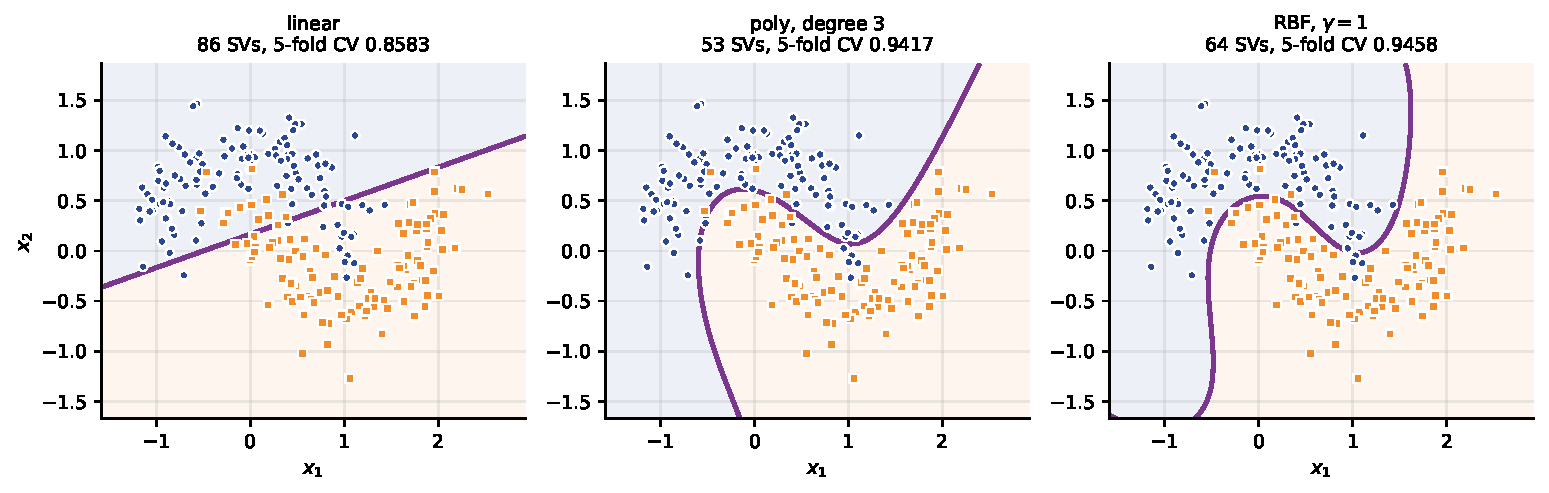
\includegraphics[width=0.94\textwidth]{kernels.pdf}
  \caption{Decision boundaries of the four kernels on the two-moons problem.
  Linear cannot bend; degree two bends the wrong way; degree three and the RBF
  both find the crescent shape.}
  \label{fig:kernels}
\end{figure}

Read the second row carefully, because it is the honest one. \textbf{The
degree-two polynomial is worse than the plain linear kernel} --- $0.8417$
against $0.8583$ in cross-validation. An even-degree polynomial kernel is
symmetric in a way that this data is not, so the extra flexibility is spent in
the wrong direction. More flexibility is not automatically better; it has to be
the \emph{right} flexibility. This is why kernel choice is a hyperparameter to
be validated and not a preference to be asserted.

\begin{caution}[Not every function is a kernel]
$K$ must be a valid inner product in \emph{some} space, which by Mercer's
condition means the Gram matrix $[K(x_i,x_j)]$ must be symmetric positive
semi-definite for every finite sample. Linear, polynomial and RBF all satisfy
this. The ``sigmoid kernel'' $\tanh(\gamma x^\top z + r)$, which scikit-learn
also offers, does \emph{not} for all parameter settings, and \texttt{libsvm}
may then fail to converge or return nonsense. Do not invent a similarity
function and pass it as a kernel without checking.
\end{caution}

% =========================================================================
\section{$\gamma$, scaling and what it all costs}
\label{sec:gamma}

\subsection{$\gamma$ is how far one training point reaches}

For the RBF kernel, $K(x_i, x)$ is the influence that training point $x_i$ has
at the query point $x$, and it decays with distance at a rate set by $\gamma$.
A useful way to make that concrete is to ask at what distance the influence has
fallen to $1\%$: solving $e^{-\gamma r^2} = 0.01$ gives
$r = \sqrt{-\ln(0.01)/\gamma}$.

\begin{lstlisting}
print(" gamma   distance at which K falls to 0.01   nSV   train   5-fold CV")
for g in [0.01, 0.1, 1.0, 10.0, 100.0]:
    reach = np.sqrt(-np.log(0.01) / g)
    c = SVC(kernel="rbf", gamma=g, C=1.0).fit(Xm, ym)
    cv = cross_val_score(SVC(kernel="rbf", gamma=g, C=1.0), Xm, ym, cv=CV).mean()
    print("%6g            %8.4f              %3d   %.4f   %.4f"
          % (g, reach, c.n_support_.sum(), c.score(Xm, ym), cv))
\end{lstlisting}
\begin{codeout}
 gamma   distance at which K falls to 0.01   nSV   train   5-fold CV
  0.01             21.4597              158   0.8208   0.8167
   0.1              6.7861              103   0.8542   0.8542
     1              2.1460               64   0.9583   0.9458
    10              0.6786               89   0.9708   0.9625
   100              0.2146              212   0.9917   0.9125
\end{codeout}

\begin{figure}[tb]
  \centering
  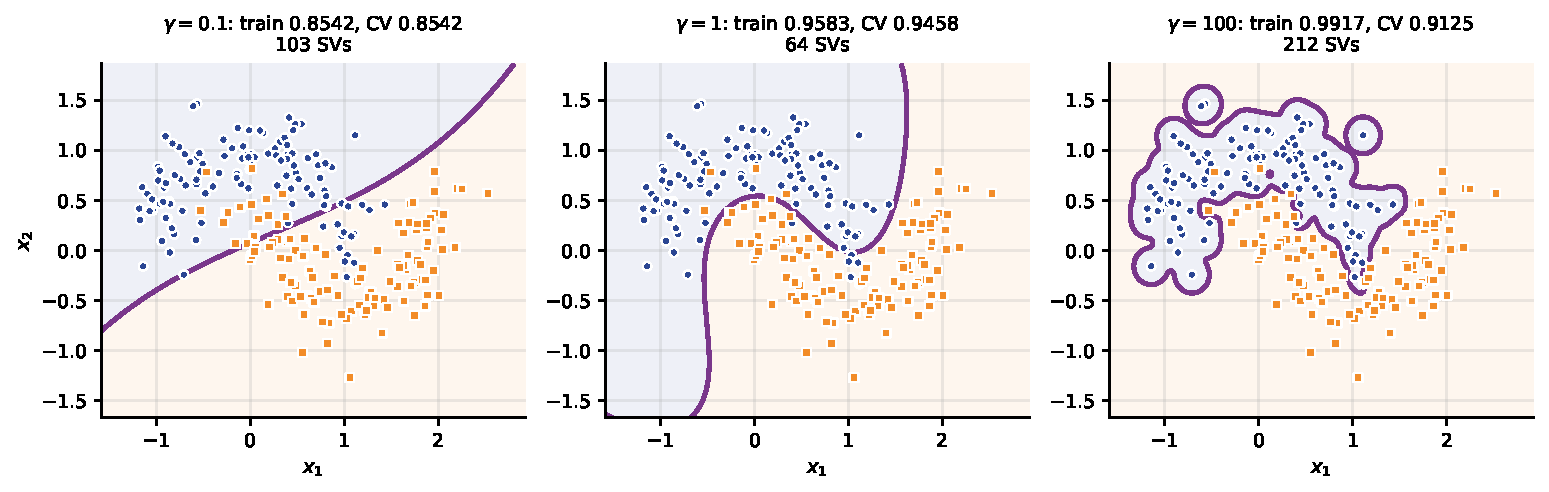
\includegraphics[width=0.94\textwidth]{gammaboundary.pdf}
  \caption{RBF decision boundaries on two moons at increasing $\gamma$. Small
  $\gamma$: every point influences the whole plane and the boundary is nearly
  straight. Large $\gamma$: influence dies within $0.21$ units, so the model
  builds a small island around each training point.}
  \label{fig:gammaboundary}
\end{figure}

The whole dataset spans about three units, so a reach of $21.46$ at
$\gamma = 0.01$ means every point influences every other point equally: the
model degenerates towards a straight line and scores $0.8167$. A reach of
$0.2146$ at $\gamma = 100$ means a point influences essentially only itself,
and the model becomes a lookup table --- training accuracy $0.9917$,
cross-validated $0.9125$, with $212$ of $240$ points recruited as support
vectors.

\begin{keyidea}
$C$ and $\gamma$ control different things and both matter. $C$ is how much
violation you tolerate; $\gamma$ is how far one training example's influence
extends. Small $\gamma$ underfits towards linearity, large $\gamma$ overfits
towards memorisation, and there is no default that is right for every dataset.
Search over both, on a logarithmic grid.
\end{keyidea}

\subsection{Large $\gamma$ overfits, and it is spectacular}

Two moons is a toy. The same failure on real data is worth seeing because of
how extreme it gets.

\begin{lstlisting}
print("  gamma    train    5-fold CV    nSV of 569")
for g in [0.001, 0.01, 0.1, 1.0, 10.0]:
    p = make_pipeline(StandardScaler(), SVC(kernel="rbf", gamma=g, C=1.0))
    tr = p.fit(Xc, yc).score(Xc, yc)
    cv = cross_val_score(make_pipeline(StandardScaler(),
                                       SVC(kernel="rbf", gamma=g, C=1.0)),
                         Xc, yc, cv=CV).mean()
    print("%7g    %.4f    %.4f       %d" % (g, tr, cv, p[-1].n_support_.sum()))
print("majority class = %.4f" % max(yc.mean(), 1 - yc.mean()))
\end{lstlisting}
\begin{codeout}
  gamma    train    5-fold CV    nSV of 569
  0.001    0.9525    0.9455       200
   0.01    0.9824    0.9701       111
    0.1    0.9912    0.9596       221
      1    1.0000    0.6309       568
     10    1.0000    0.6274       569
majority class = 0.6274
\end{codeout}

At $\gamma = 10$ the training accuracy is $\mathbf{1.0000}$ and the
cross-validated accuracy is $\mathbf{0.6274}$ --- \emph{exactly} the
majority-class rate, to four decimals. And $\mathbf{569}$ of $569$ rows are
support vectors: the model has stored the entire training set and generalises
to nothing. It answers every new query by finding that nothing in its memory is
close enough to matter and falling back on the intercept.

\begin{figure}[tb]
  \centering
  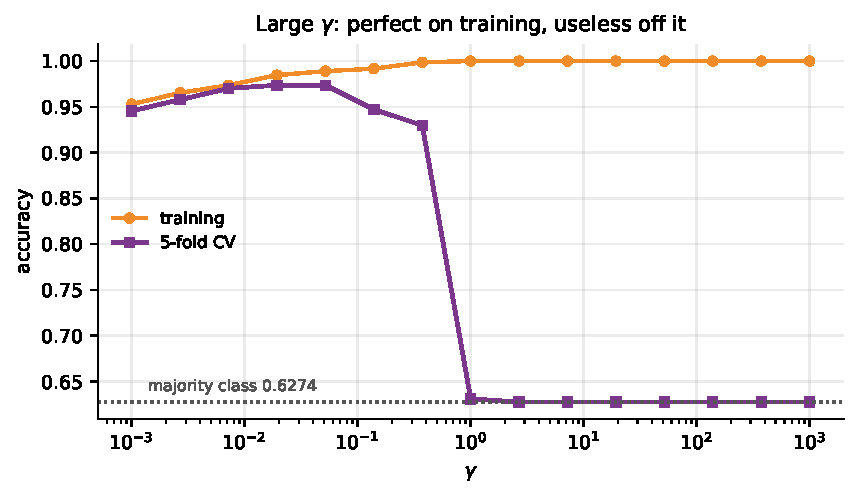
\includegraphics[width=0.62\textwidth]{gammacurve.pdf}
  \caption{Training and cross-validated accuracy against $\gamma$ on scaled
  \texttt{breast\_cancer}. The training curve reaches $1.0000$ and stays; the
  validation curve collapses to the majority-class rate. The best
  cross-validated point is in the middle, at $\gamma = 0.01$.}
  \label{fig:gammacurve}
\end{figure}

\begin{caution}[A perfect training score from an SVM is a warning, not a result]
Any RBF SVM can reach training accuracy $1.0000$ by taking $\gamma$ large
enough, on any dataset, including one with random labels. Reporting it as an
achievement is the classic error. Watch the \emph{gap} between the training and
validation curves; a gap of $0.3726$ is what memorisation looks like.
\end{caution}

\subsection{Scaling is mandatory}

Look at \eqref{eq:rbf} again. The kernel depends on the data only through
$\|x - z\|^2 = \sum_k (x_k - z_k)^2$, an unweighted sum over the columns. If
one column is measured in thousands and another in thousandths, the first
column contributes essentially the whole of that sum and the RBF kernel
effectively sees a one-feature problem.

\begin{lstlisting}
sd = Xc.std(0)
print("breast_cancer: widest column sd %.4f, narrowest %.6f, ratio %.1f"
      % (sd.max(), sd.min(), sd.max() / sd.min()))
setups = [("SVC(rbf, gamma='scale')", SVC(kernel="rbf", gamma="scale")),
          ("SVC(rbf, gamma=1)",       SVC(kernel="rbf", gamma=1.0)),
          ("SVC(linear)",             SVC(kernel="linear")),
          ("SVC(poly, degree 3)",     SVC(kernel="poly", degree=3))]
print("%-26s %8s %8s %8s" % ("model", "raw", "scaled", "gap"))
for nm, est in setups:
    r = cross_val_score(est, Xc, yc, cv=CV).mean()
    s = cross_val_score(make_pipeline(StandardScaler(), est), Xc, yc, cv=CV).mean()
    print("%-26s %8.4f %8.4f %+8.4f" % (nm, r, s, s - r))
\end{lstlisting}
\begin{codeout}
breast_cancer: widest column sd 568.8565, narrowest 0.002644, ratio 215170.7
model                           raw   scaled      gap
SVC(rbf, gamma='scale')      0.9210   0.9771  +0.0561
SVC(rbf, gamma=1)            0.6274   0.6309  +0.0035
SVC(linear)                  0.9526   0.9754  +0.0229
SVC(poly, degree 3)          0.9122   0.8981  -0.0142
\end{codeout}

The column standard deviations on this dataset differ by a factor of
$\mathbf{215\,171}$. Standardising before an RBF SVM is worth
$\mathbf{+0.0561}$ of cross-validated accuracy --- fifty-six patients in a
thousand, given away by one missing line of code.

\begin{figure}[tb]
  \centering
  
\includegraphics[width=0.68\textwidth]{scaling.pdf}
  \caption{Five-fold cross-validated accuracy on \texttt{breast\_cancer}, raw
  against standardised, for four SVMs. The dotted line is the majority-class
  rate. Three of the four improve; the degree-3 polynomial does not.}
  \label{fig:scaling}
\end{figure}

Report the row that disagrees. The degree-3 polynomial kernel got
\emph{worse} when scaled, by $-0.0142$. That happens, and hiding it would make
the rule sound like a theorem when it is a very reliable default. Note also
that both of its scores are below the scaled RBF anyway, so the exception does
not change what you would actually deploy.

\begin{caution}[Scale inside a \texttt{Pipeline}, never before the split]
\begin{lstlisting}
pipe = make_pipeline(StandardScaler(), SVC(kernel="rbf"))   # correct
Xall = StandardScaler().fit_transform(X)                    # LEAKAGE
\end{lstlisting}
Fitting the scaler on the whole table lets the test rows contribute to the
mean and standard deviation used to transform the training rows. Every
cross-validated number you then report is optimistic. Inside a
\texttt{Pipeline}, scikit-learn refits the scaler on each training fold, which
is the only correct thing to do.
\end{caution}

\subsection{The whole recipe, in six lines}

\begin{lstlisting}
Xtr, Xte, ytr, yte = train_test_split(Xc, yc, test_size=0.25,
                                      stratify=yc, random_state=0)
pipe = Pipeline([("scale", StandardScaler()), ("svm", SVC(kernel="rbf"))])
grid = {"svm__C": [0.1, 1, 10, 100], "svm__gamma": [0.001, 0.01, 0.1, 1]}
gs = GridSearchCV(pipe, grid, cv=CV, n_jobs=1).fit(Xtr, ytr)
\end{lstlisting}
\begin{codeout}
best parameters : {'svm__C': 100, 'svm__gamma': 0.001}
best CV score   : 0.9859
held-out score  : 0.9580
support vectors : 43 of 426 training rows
\end{codeout}

Three things to notice. The chosen configuration pairs a \emph{large} $C$ with
a \emph{tiny} $\gamma$ --- the two parameters trade off against each other,
which is why they must be searched jointly rather than one at a time. The final
model uses $43$ of $426$ training rows. And the held-out score, $0.9580$, is
\emph{below} the cross-validated score, $0.9859$. That gap is the optimism of
having chosen the best of sixteen configurations on the same folds you are
quoting. \textbf{Report the held-out number.}

\subsection{What it costs as the data grows}
\label{sec:cost}

Everything so far has been on datasets of a few hundred rows. The following
sweep goes to thirty-two thousand rows. Count first and time second: the
support-vector counts below are exact arithmetic on a fixed dataset and are
the same on every machine, and the seconds are not.

\begin{lstlisting}
Xg, yg = make_classification(n_samples=40000, n_features=20, n_informative=8,
                             class_sep=0.9, random_state=0)   # fixes the data
Xg = StandardScaler().fit_transform(Xg)
for n in [500, 1000, 2000, 4000, 8000, 16000, 32000]:
    e = SVC(kernel="rbf").fit(Xg[:n], yg[:n])
    print(n, e.n_support_.sum(), n * n)     # exact: support vectors, kernel
\end{lstlisting}
\begin{codeout}
     n     nSV easy   nSV hard   kernel entries n^2
   500        248        380               250000
  2000        624       1097              4000000
  8000       1604       3108             64000000
 32000       4596       9280           1024000000
nSV grows as n^0.69 (class_sep 0.9) and n^0.76 (class_sep 0.4)
64x the rows gives 18.5x the support vectors on the easy problem and
24.4x on the hard one; the kernel matrix grows 4096x either way
\end{codeout}

That is the reproducible statement of the cost, and it already contains the
whole argument. The object the solver must reason about, the kernel matrix,
grows as $n^2$: $4096$ times bigger over this sweep. The object the answer
actually depends on, the support-vector set, grows only as $n^{0.69}$ --- and
the fraction of rows kept falls from $0.50$ to $0.14$. The cost sits between
those two, which is why the measured exponent comes out between $1$ and $2$.
And make the problem harder --- \texttt{class\_sep} $0.4$ instead of $0.9$ ---
so that more rows stay support vectors ($0.29$ of them at $n = 32000$ against
$0.14$), and the support-vector exponent rises from $0.69$ to $0.76$. The
cost must rise with it.

Now the clock, separately and with a health warning:

\begin{codeout}
     n   SVC(rbf) fit   nSV / n   LinearSVC fit    ratio
   500         0.003 s     0.50          0.001 s      3.6x
  2000         0.024 s     0.31          0.002 s     13.6x
  8000         0.257 s     0.20          0.005 s     47.1x
 32000         3.308 s     0.14          0.048 s     68.7x
MACHINE-DEPENDENT (one machine, one run; do not quote as a constant):
fitted exponent, SVC(rbf), class_sep 0.9 : time ~ n^1.72
fitted exponent, SVC(rbf), class_sep 0.4 : time ~ n^1.81
fitted exponent, LinearSVC               : time ~ n^0.98
\end{codeout}

\begin{caution}[Timings are the one thing a seed cannot fix]
Every other number in these notes is reproducible: fixed data, fixed seed,
same answer on your machine as on mine. The seconds above are not. They depend
on your processor, your BLAS build and what else is running, and repeated runs
on the \emph{same} machine here moved the fitted exponent between $n^{1.68}$
and $n^{1.72}$ and the $64\times$ ratio between roughly $990$ and $1210$.

So quote the counts, never the seconds. ``$64\times$ the rows gives
$18.5\times$ the support vectors and $4096\times$ the kernel matrix'' is true
on every machine; ``$3.3$ seconds at $n = 32000$'' is true on exactly one. If
you measure a different exponent, you are not wrong --- and neither is this
page.
\end{caution}

\begin{figure}[tb]
  \centering
  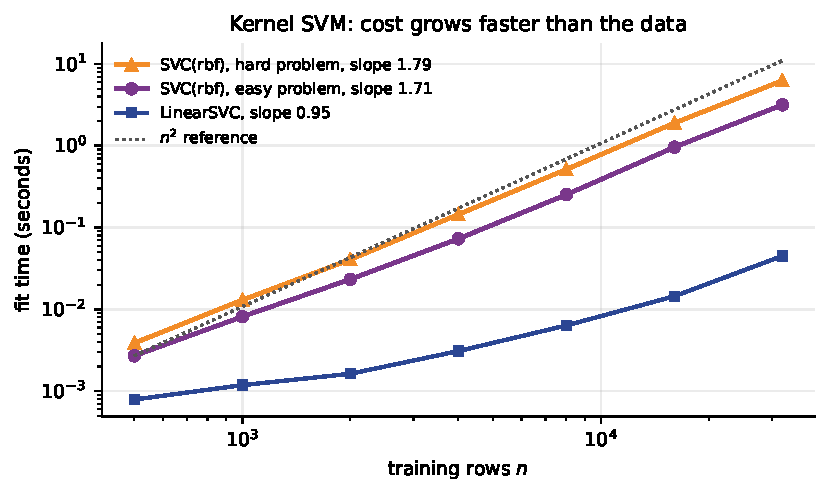
\includegraphics[width=0.62\textwidth]{cost.pdf}
  \caption{Fit time against $n$ on log-log axes for a kernel SVM on two
  problems of different difficulty, and for \texttt{LinearSVC}. A straight line
  on these axes is a power law, and its slope is the exponent.}
  \label{fig:cost}
\end{figure}

Be precise about what this shows. The textbook statement is that kernel SVM
training is between $O(n^2)$ and $O(n^3)$, since the kernel matrix alone has
$n^2$ entries. The measured exponent is \emph{below} quadratic, and the honest
thing is to say so and then explain it --- which the counts already did.
\texttt{libsvm} caches kernel rows and shrinks the active set, so the work is
driven by the support vectors rather than by the rows, and the support-vector
count grows far more slowly than $n$. The check on that explanation is the
second problem: keep more rows as support vectors and both the count exponent
and the time exponent rise together, in the predicted direction.

The practical conclusion survives intact either way, and it should be stated
in counts. \textbf{Sixty-four times the rows gives $18.5\times$ the support
vectors and $4096\times$ the kernel matrix}, and on the machine that built
this lecture that came to roughly a thousandfold in seconds. Extrapolating
that growth from thirty-two thousand rows to one million puts a single fit in
the region of an hour, and a grid search over sixteen configurations with five
folds multiplies that by eighty.

\begin{keyidea}[When not to use a kernel SVM]
Past roughly $10^5$ rows, do not. Use \texttt{LinearSVC} --- measured at
essentially linear scaling here, and it never forms a kernel matrix at all
--- or \texttt{SGDClassifier} with
\texttt{loss='hinge'}, which minimises the same objective
\eqref{eq:hingeobj} one row at a time and scales to data that does not fit in
memory. You give up the non-linear boundary; you get a model that finishes.
\end{keyidea}

\subsection{Prediction is not free either}

\begin{codeout}
C =   0.01  nSV =  5988  kernel evaluations to score 8000 rows = 47904000
           machine-dependent: 8000 rows scored in 1.528 s
C =      1  nSV =  1604  kernel evaluations to score 8000 rows = 12832000
           machine-dependent: 8000 rows scored in 0.408 s
C =    100  nSV =  1368  kernel evaluations to score 8000 rows = 10944000
           machine-dependent: 8000 rows scored in 0.349 s
\end{codeout}

Every prediction is a sum over the support vectors,
$f(x) = \sum_{i \in \mathrm{SV}} \alpha_i y_i K(x_i, x) + b$, so scoring
$8000$ rows costs exactly $8000 \times n_{\mathrm{SV}}$ kernel evaluations:
$47\,904\,000$ at $C = 0.01$ against $10\,944\,000$ at $C = 100$. That is a
count, not a clock, and it is $4.4\times$ on any machine. The seconds beside
it happen to agree. An RBF
SVM is best understood as a \emph{learned, weighted, sparse nearest-neighbour
rule}: it chooses which stored examples to keep and how much to weight them,
and then it pays k-NN's prediction-time cost on the ones it kept. If your
deployment budget is per-request latency, the support-vector count is the
number to watch, and a larger $C$ --- which keeps fewer of them --- may be
worth a little accuracy.

\subsection{More than two classes}

An SVM is intrinsically a two-class machine: one hyperplane has two sides.
scikit-learn's \texttt{SVC} handles $k$ classes by fitting $k(k-1)/2$
one-against-one machines and taking a vote.

\begin{codeout}
classes            : 3
pairwise SVMs      : 3  (= k(k-1)/2)
dual_coef_ shape   : (2, 51)
n_support_ per class: [ 8 22 21]
decision_function  : (1, 3) one column per pair
5-fold CV accuracy : 0.9533
\end{codeout}

Three classes give three pairwise machines. At $k = 10$ --- \texttt{load\_digits},
for example --- that is $45$ models, each of which has to be fitted and each of
which has to be evaluated at prediction time. Combined with the fit-time
scaling above, this is why kernel SVMs are rarely the first choice for
large multi-class problems.

% =========================================================================
\section{Summary}
\label{sec:summary}

\begin{enumerate}[leftmargin=*]
  \item \textbf{Accuracy cannot rank perfect classifiers.} Of five lines that
    each got all six points right, the clearance ranged from $0.0707$ to
    $\mathbf{0.7071}$ --- a factor of ten, invisible to any metric computed
    from predictions.
  \item \textbf{The geometry.} The signed distance to $w^\top x + b = 0$ is
    $(w^\top x + b)/\|w\|$. Fix the scale so the closest points have
    $y_i f(x_i) = 1$ and the empty band has width $\mathbf{2/\|w\|}$.
    Maximising it is minimising $\tfrac12\|w\|^2$ subject to
    $y_i(w^\top x_i + b) \ge 1$: a convex quadratic program with one global
    optimum.
  \item \textbf{The dual.} The Lagrangian gives $w = \sum_i \alpha_i y_i x_i$
    and $\sum_i \alpha_i y_i = 0$; substituting yields a maximisation in
    $\alpha$ in which the data appears \textbf{only} as
    $\langle x_i, x_j\rangle$.
  \item \textbf{Support vectors, earned not announced.} Complementary
    slackness $\alpha_i[y_i f(x_i) - 1] = 0$ forces every point to have either
    $\alpha_i = 0$ or $y_i f(x_i) = 1$. The latter are the support vectors and
    the model is built from them alone.
  \item \textbf{Six points by hand.} $\alpha_A = \alpha_D = 1$, $w = (1,1)$,
    $b = -3$, width $\mathbf{1.414214}$; \texttt{SVC(kernel='linear', C=1e6)}
    returns the identical numbers to $10^{-9}$, and the dual objective
    $1.0000000000$ equals $\tfrac12\|w\|^2 = 1.0000000000$.
  \item \textbf{Deletion.} Deleting non-support-vector $B$ moved $w$ by
    $\mathbf{0.00\mathrm{e}{+}00}$ and $b$ by $0.00\mathrm{e}{+}00$. Deleting
    support vector $A$ moved $w$ to $(0.6664, 0.6668)$ and widened the margin
    to $2.1215$ --- matching the hand calculation $1.5\sqrt2 = 2.1213$.
    Refitting on the $11$ support vectors of an $80$-point problem gave
    identical predictions on all $80$; the other $69$ rows changed nothing.
  \item \textbf{Soft margin.} $\xi_i \ge 0$, objective
    $\tfrac12\|w\|^2 + C\sum_i \xi_i$, dual unchanged except
    $0 \le \alpha_i \le C$. Across $C = 0.01 \to 1000$ the width went
    $5.2135 \to 1.3483$ and the points inside the margin $32 \to 5$, while
    training accuracy stayed at $0.9625$ in every row.
  \item \textbf{$C$ is inverse regularisation.} Dividing the objective by $C$
    puts $1/(2C)$ on $\|w\|^2$, so $\lambda = 1/C$. Measured: $\|w\|$ climbed
    $0.3555 \to 20.8998$ as $C$ went $0.001 \to 100$, and cross-validated
    accuracy peaked at $\mathbf{0.9772}$ in the middle, at $C = 0.1$.
  \item \textbf{The hinge.} Eliminating $\xi$ gives
    $\sum_i \max(0, 1 - y_i f(x_i)) + \frac{1}{2C}\|w\|^2$: the SVM is the
    model whose loss is the hinge of the loss-functions lecture. It is exactly
    zero beyond $m = 1$, which is why most $\alpha_i$ vanish --- $11$ of $80$
    points had $m \le 1$ and \texttt{n\_support\_} was $11$. Against logistic
    regression: $40$ rows used against $569$, cosine $0.9132$, CV $0.9754$
    against $0.9789$.
  \item \textbf{Kernels.}
    $\langle\varphi(x),\varphi(z)\rangle = (1 + x^\top z)^2$ verified to
    $0.00\mathrm{e}{+}00$ at $x = (1,2)$, $z = (3,1)$ (both sides $36$), and to
    $2.842\times10^{-14}$ over a $200\times200$ Gram matrix. Kernel machine and
    explicit-map machine agree to $1.24\times10^{-14}$ with the same $38$
    support vectors. Circles: $0.5682 \to \mathbf{1.0000}$. At $d = 100$,
    degree $5$, the explicit map has $96\,560\,646$ columns and the kernel
    costs $d+1$ multiplications.
  \item \textbf{$\gamma$ and scaling.} $\gamma$ is a reach: influence falls to
    $1\%$ at $\sqrt{-\ln(0.01)/\gamma}$. On \texttt{breast\_cancer},
    $\gamma = 10$ gives training $1.0000$, CV $\mathbf{0.6274}$ --- exactly the
    majority-class rate --- with $569/569$ rows as support vectors. Without
    \texttt{StandardScaler} the RBF SVM loses $\mathbf{0.0561}$; the column
    standard deviations differ by a factor of $215\,171$.
  \item \textbf{Cost, in counts.} $64\times$ the rows gives $18.5\times$ the
    support vectors ($n_{\mathrm{SV}} \sim n^{0.69}$) and $4096\times$ the
    kernel matrix, and the support-vector fraction falls from $0.50$ to
    $0.14$. That is why the measured \emph{time} exponent comes out below the
    documented $O(n^2)$--$O(n^3)$. Prediction is a count too: scoring $8000$
    rows costs $8000\,n_{\mathrm{SV}}$ kernel evaluations, $4.4\times$ more
    at $C = 0.01$ than at $C = 100$. Past $\sim 10^5$ rows use
    \texttt{LinearSVC}, which never forms the kernel matrix, or
    \texttt{SGDClassifier}.
\end{enumerate}

% =========================================================================
\section{Practice questions}
\label{sec:questions}

Work these with a pen before running anything. Solutions with full working
follow in Section~\ref{sec:solutions}.

\begin{enumerate}[leftmargin=*]
  \item \textbf{Geometric margins by hand.} A linear classifier has
    $w = (3, 4)$ and $b = -10$. Four points are given:
    $P_1 = (1,1)$ with $y = -1$, $P_2 = (2,2)$ with $y = +1$,
    $P_3 = (4,1)$ with $y = +1$, and $P_4 = (0,3)$ with $y = +1$.
    (a) Compute the signed distance of each point from the boundary.
    (b) Compute each functional margin $y_i f(x_i)$ and each geometric margin.
    (c) Which point is nearest the boundary, and what is the width of the
    largest empty band centred on this particular line? (d) Is $(w,b)$ in
    canonical form for this dataset? If not, give the scale factor that makes
    it so.

  \item \textbf{Two points, solved completely.} A training set has exactly two
    points: $x_- = (2,1)$ with $y = -1$ and $x_+ = (4,3)$ with $y = +1$.
    Working from $w = \sum_i \alpha_i y_i x_i$ and $\sum_i \alpha_i y_i = 0$,
    find $\alpha$, $w$, $b$ and the margin width. Verify that both functional
    margins equal $1$, and check your margin width against
    $\|x_+ - x_-\|$. Explain why those last two numbers must agree.

  \item \textbf{Six points, solved completely.} Negatives $A = (1,1)$,
    $B = (0,1)$, $C = (1,0)$; positives $D = (3,3)$, $E = (4,3)$, $F = (3,4)$.
    (a) Identify the support vectors by inspection and justify the choice.
    (b) Find $w$, $b$ and both multipliers. (c) Compute $y_i f(x_i)$ for all
    six points and confirm the guess. (d) Give the margin width. (e) State
    what happens to $w$, $b$ and the width if $E$ is deleted, and why you know
    without refitting.

  \item \textbf{Canonical rescaling.} Someone hands you $w = (2,2)$,
    $b = -6$ for the six points of Section~\ref{sec:sixpoints}.
    (a) Compute $\min_i y_i(w^\top x_i + b)$. (b) Is this the canonical form?
    (c) Give the $c > 0$ for which $(cw, cb)$ is canonical, and confirm that
    $2/\|cw\|$ then equals the margin width reported in the notes.
    (d) Explain in one sentence why $\tfrac12\|w\|^2$ is a legitimate objective
    only once the normalisation is fixed.

  \item \textbf{Slacks and the objective.} Five points have functional margins
    $m_i = y_i f(x_i)$ equal to $2.3$, $1.0$, $0.4$, $-0.6$ and $1.7$.
    (a) Compute each $\xi_i$. (b) Classify each point into the three regimes of
    Section~\ref{sec:soft}. (c) How many are misclassified? (d) If
    $\|w\| = 2$ and $C = 0.5$, compute the soft-margin objective.
    (e) Which of these points have $\alpha_i > 0$, and which are at the
    ceiling $\alpha_i = C$?

  \item \textbf{A kernel identity, verified.} Take $x = (2,0)$ and
    $z = (1,1)$, and the degree-2 map $\varphi$ of equation \eqref{eq:phi2}.
    (a) Compute $(1 + \langle x, z\rangle)^2$. (b) Write out $\varphi(x)$ and
    $\varphi(z)$ and compute their inner product term by term. (c) State how
    many multiplications each route needed. (d) Explain what would go wrong
    with the identity if the $\sqrt2$ factors were dropped from $\varphi$.

  \item \textbf{The RBF as a similarity.} Let $\gamma = 0.5$, $u = (1,2)$,
    $v = (2,4)$. (a) Compute $\|u - v\|^2$ and $K(u,v)$. (b) At what distance
    does $K$ fall to $0.01$? (c) If every feature were multiplied by $10$
    (say, a change of units from centimetres to millimetres), what would
    $K(u,v)$ become, and what does that tell you about scaling? (d) Why is
    there no explicit feature map to write down for this kernel?

  \item \textbf{Reading a $C$ sweep.} A classmate reports: ``I swept $C$ and
    got training accuracy $0.94$, $0.97$, $0.99$, $1.00$, $1.00$ for
    $C = 0.01, 0.1, 1, 10, 100$, so $C = 100$ is best, and since large $C$
    regularises more, my model is nicely constrained.'' Identify every error
    in that sentence, say what you would ask them to compute instead, and
    predict --- using the table of Section~\ref{sec:invreg} --- roughly what
    they would find.

  \item \textbf{Choosing a route.} You have a text-classification problem:
    $n = 3000$ documents, $d = 50\,000$ TF--IDF columns, two classes,
    approximately linearly separable. Your colleague proposes an RBF SVM with a
    grid over $C$ and $\gamma$. (a) Would you use the primal or the dual, and
    why, on these dimensions? (b) How many features would a degree-3 explicit
    polynomial map have here, and is that a problem for a kernel method?
    (c) Would you standardise? (d) What would you actually run?

  \item \textbf{The scaling budget.} A production system has $1.2$ million
    labelled rows and $60$ features, and you must retrain nightly within a
    two-hour window. Using the measured exponents of Section~\ref{sec:cost},
    estimate the fit time of a single \texttt{SVC(kernel='rbf')} on the full
    data, taking as your anchor the $3.308$ seconds that $32\,000$ rows took
    on the machine that built these notes. Then estimate the cost of a
    $4 \times 4$ grid search with five-fold cross-validation. State what you
    would do instead and what you would lose by doing it --- and say in one
    sentence why the answer is an order of magnitude rather than a number.
\end{enumerate}

% =========================================================================
\section{Solutions}
\label{sec:solutions}

\paragraph{1. Geometric margins by hand.}
$\|w\| = \sqrt{3^2 + 4^2} = 5$, which is why these numbers were chosen.

(a) $f(x) = 3x_1 + 4x_2 - 10$, and the signed distance is $f(x)/5$:
\[
  \begin{array}{lrrr}
    \text{point} & f(x) & f(x)/\|w\| & y \\
    P_1 = (1,1) & 3 + 4 - 10 = -3 & -0.6 & -1\\
    P_2 = (2,2) & 6 + 8 - 10 = +4 & +0.8 & +1\\
    P_3 = (4,1) & 12 + 4 - 10 = +6 & +1.2 & +1\\
    P_4 = (0,3) & 0 + 12 - 10 = +2 & +0.4 & +1
  \end{array}
\]

(b) Functional margins $y_i f(x_i)$: $(-1)(-3) = 3$, $4$, $6$, $2$. Geometric
margins are these divided by $5$: $0.6$, $0.8$, $1.2$, $\mathbf{0.4}$. All are
positive, so all four points are correctly classified.

(c) The nearest point is $P_4$ at $0.4$. The widest empty band centred on
\emph{this} line has half-width $0.4$ and therefore width $\mathbf{0.8}$. Note
this is a property of the line we were given, not the maximum-margin line: some
other line through this data would do better.

(d) No. Canonical form requires $\min_i y_i f(x_i) = 1$ and here the minimum
is $2$. Dividing by $2$ gives $c = 1/2$, so $w' = (1.5, 2)$, $b' = -5$, and
then $\|w'\| = 2.5$ and $2/\|w'\| = 0.8$ --- the same width as in (c), which is
the point of the normalisation: it changes the numbers on the page and not the
geometry.

\paragraph{2. Two points, solved completely.}
With two points, one of each class, \eqref{eq:sumzero} reads
$-\alpha_- + \alpha_+ = 0$, so $\alpha_- = \alpha_+ = \alpha$, and
\eqref{eq:wsum} gives
\[
  w = \alpha\bigl[(4,3) - (2,1)\bigr] = \alpha\,(2,2) .
\]
Both points are support vectors, so both satisfy $y_i f(x_i) = 1$:
\[
  \text{$x_+$:}\ \ 4\cdot 2\alpha + 3\cdot 2\alpha + b = 1
  \;\Rightarrow\; 14\alpha + b = 1 ,
  \qquad
  \text{$x_-$:}\ \ -(2\cdot 2\alpha + 1\cdot 2\alpha + b) = 1
  \;\Rightarrow\; -6\alpha - b = 1 .
\]
Adding: $8\alpha = 2$, so $\alpha = 0.25$, giving
\[
  w = 0.25\,(2,2) = \mathbf{(0.5,\, 0.5)},
  \qquad
  b = 1 - 14(0.25) = \mathbf{-2.5} .
\]
Check the functional margins: $f(x_-) = 1 + 0.5 - 2.5 = -1$, so
$y_- f(x_-) = 1$; $f(x_+) = 2 + 1.5 - 2.5 = +1$, so $y_+ f(x_+) = 1$. Both
equal $1$, as required.

Width: $\|w\| = \sqrt{0.25 + 0.25} = 1/\sqrt2$, so
$2/\|w\| = 2\sqrt2 = \mathbf{2.828427}$. And
$\|x_+ - x_-\| = \|(2,2)\| = 2\sqrt2 = 2.828427$.

They must agree because with exactly one support vector on each side there is
nothing else constraining the band: the widest slab separating two single
points is the one perpendicular to the segment joining them, with each point on
one edge, and its width is the length of that segment. The general formula
$w = 2(x_+ - x_-)/\|x_+ - x_-\|^2$ falls straight out of this. Running the
computation confirms it:

\begin{codeout}
difference vector    : [2. 2.]
w = 2(x+ - x-)/||.||^2 = [0.5 0.5]
b                    = -2.5000
margins y f(x)       : [1. 1.]
2/||w||              = 2.828427
||x+ - x-||          = 2.828427
SVC                  : w = [0.5 0.5]  b = -2.500000
\end{codeout}

\paragraph{3. Six points, solved completely.}
(a) The two points closest across the class boundary are $A = (1,1)$ and
$D = (3,3)$, at distance $2\sqrt2 \approx 2.83$; every other cross-class pair
is further apart ($B$ to $D$ is $\sqrt{13} \approx 3.61$, for instance). The
maximum-margin boundary is determined by the closest opposing points, so
$\{A, D\}$ is the natural guess for the support set.

(b) Since one support vector lies on each side, Question 2's formula applies
directly with $x_- = A$, $x_+ = D$ and $x_+ - x_- = (2,2)$:
\[
  w = \frac{2(2,2)}{\|(2,2)\|^2} = \frac{2(2,2)}{8} = \mathbf{(0.5,\,0.5)} .
\]
Both are on the margin, so $b = 1 - w^\top D = 1 - (1.5 + 1.5) = \mathbf{-2}$.
And from $w = \alpha[(3,3)-(1,1)] = \alpha(2,2) = (0.5,0.5)$ we get
$\alpha_A = \alpha_D = \mathbf{0.25}$.

(c) With $f(x) = 0.5x_1 + 0.5x_2 - 2$:
\[
  \begin{array}{lrrl}
    A(1,1) & f = -1.0 & y f = 1.0 & \text{on the margin}\\
    B(0,1) & f = -1.5 & y f = 1.5 & \text{outside}\\
    C(1,0) & f = -1.5 & y f = 1.5 & \text{outside}\\
    D(3,3) & f = +1.0 & y f = 1.0 & \text{on the margin}\\
    E(4,3) & f = +1.5 & y f = 1.5 & \text{outside}\\
    F(3,4) & f = +1.5 & y f = 1.5 & \text{outside}
  \end{array}
\]
Every constraint $y_i f(x_i) \ge 1$ holds, and exactly two hold with equality,
so the guess was correct.

(d) $\|w\| = 1/\sqrt2$, so the width is $2\sqrt2 = \mathbf{2.828427}$ --- which
is $\|D - A\|$, as it must be.

(e) Nothing happens. $E$ has $\alpha_E = 0$, so by \eqref{eq:wsum} it does not
appear in $w$ at all, and its constraint is slack ($1.5 > 1$) so removing it
does not free anything up. Both $w$ and $b$ are unchanged and the width stays
at $2.828427$. You do not need to refit to know this; that is the content of
complementary slackness.

\paragraph{4. Canonical rescaling.}
(a) With $w = (2,2)$, $b = -6$ we have $f(x) = 2x_1 + 2x_2 - 6$, so
$f(A) = -2$, $f(B) = f(C) = -4$, $f(D) = +2$, $f(E) = f(F) = +4$. The
functional margins are $2, 4, 4, 2, 4, 4$, so
$\min_i y_i f(x_i) = \mathbf{2}$.

(b) No: canonical form requires that minimum to be $1$.

(c) Take $c = 1/2$. Then $cw = (1,1)$ and $cb = -3$, which is exactly the
solution of Section~\ref{sec:hand}, and
$2/\|cw\| = 2/\sqrt2 = 1.414214$ --- the margin width reported there.

(d) Because $\tfrac12\|w\|^2$ can be driven to zero by scaling $(w,b)$ down,
which changes no prediction whatsoever. Minimising it is only meaningful once
the constraints $y_i(w^\top x_i + b) \ge 1$ pin the scale, and those
constraints are precisely the canonical normalisation written as inequalities.

\paragraph{5. Slacks and the objective.}
(a) $\xi_i = \max(0, 1 - m_i)$:
\[
  \xi = (0,\ 0,\ 0.6,\ 1.6,\ 0),
  \qquad \textstyle\sum_i \xi_i = \mathbf{2.2} .
\]

(b) $m = 2.3$: outside the margin, $\xi = 0$, a spectator. $m = 1.0$: exactly
\emph{on} the margin, $\xi = 0$. $m = 0.4$: inside the band but correctly
classified, $0 < \xi \le 1$. $m = -0.6$: past the boundary,
$\xi = 1.6 > 1$, misclassified. $m = 1.7$: outside, $\xi = 0$.

(c) One --- the point with $m = -0.6$. A point is misclassified exactly when
$m < 0$, equivalently $\xi > 1$.

(d) $\tfrac12\|w\|^2 + C\sum\xi_i
   = \tfrac12(4) + 0.5(2.2) = 2 + 1.1 = \mathbf{3.1}$.

(e) By complementary slackness, $\alpha_i > 0$ requires $m_i \le 1$: that is
the three points with $m = 1.0$, $0.4$ and $-0.6$. Of these, the two with
$\xi_i > 0$ (the ones at $0.4$ and $-0.6$) are pinned at the ceiling
$\alpha_i = C = 0.5$, and the one sitting exactly on the margin has
$0 < \alpha_i < C$. The two with $m > 1$ have $\alpha_i = 0$.

\paragraph{6. A kernel identity, verified.}
(a) $\langle x, z\rangle = 2\cdot1 + 0\cdot1 = 2$, so
$(1 + 2)^2 = \mathbf{9}$.

(b) From \eqref{eq:phi2},
\[
  \varphi(2,0) = \bigl(1,\ 2\sqrt2,\ 0,\ 4,\ 0,\ 0\bigr),
  \qquad
  \varphi(1,1) = \bigl(1,\ \sqrt2,\ \sqrt2,\ 1,\ 1,\ \sqrt2\bigr).
\]
Term by term:
$1\cdot1 = 1$;
$2\sqrt2\cdot\sqrt2 = 4$;
$0\cdot\sqrt2 = 0$;
$4\cdot1 = 4$;
$0\cdot1 = 0$;
$0\cdot\sqrt2 = 0$. Total $1 + 4 + 0 + 4 + 0 + 0 = \mathbf{9}$. The two agree.

(c) The kernel route: $2$ multiplications for the dot product, plus one
squaring --- three in all. The explicit route: building each six-vector costs
several multiplications, and the six-dimensional dot product costs $6$ more.
For $d = 2$ this is a trivial difference; the point of the exercise is that the
kernel cost is $O(d)$ regardless of degree while the explicit cost is
$O\bigl(\binom{d+p}{p}\bigr)$.

(d) The identity would fail. Expanding $(1 + x_1z_1 + x_2z_2)^2$ produces cross
terms with binomial coefficients $2$ --- for instance $2x_1z_1x_2z_2$ --- and
the $\sqrt2$ factors are there so that the product
$(\sqrt2 x_1x_2)(\sqrt2 z_1z_2)$ reproduces exactly that $2$. Drop them and the
left-hand side is short by those cross terms. In this particular example the
mismatch is hidden, because $x_2 = 0$ kills the affected terms; try
$x = (1,2)$, $z = (3,1)$ instead and you get $22$ instead of $36$.

\paragraph{7. The RBF as a similarity.}
(a) $u - v = (-1, -2)$, so $\|u - v\|^2 = 1 + 4 = 5$, and
\[
  K(u,v) = e^{-0.5 \times 5} = e^{-2.5} = \mathbf{0.082085} .
\]

(b) Solve $e^{-0.5 r^2} = 0.01$: $r^2 = -\ln(0.01)/0.5 = 4.60517/0.5 = 9.21034$,
so $r = \mathbf{3.034854}$.

(c) Multiplying every feature by $10$ multiplies $\|u-v\|^2$ by $100$, giving
$500$, so $K$ becomes $e^{-250} \approx 2.7\times10^{-109}$ --- numerically
zero. Every pair of points becomes mutually invisible and the kernel matrix
degenerates to the identity, at which point the SVM can do nothing but
memorise. This is the mechanism behind the $+0.0561$ of
Section~\ref{sec:gamma}: a fixed $\gamma$ is only meaningful relative to the
typical inter-point distance, which is exactly what standardisation
stabilises. It is also why the default \texttt{gamma='scale'} divides by the
feature variance --- a partial defence, not a substitute for scaling.

(d) Because $e^{t} = \sum_{k \ge 0} t^k/k!$ has infinitely many terms, so the
implied feature map has infinitely many coordinates. There is no finite vector
to write down. The kernel is computable anyway, because computing
$\langle \varphi(x), \varphi(z)\rangle$ never requires computing
$\varphi$.

\paragraph{8. Reading a $C$ sweep.}
Three errors, of increasing seriousness.

First, \textbf{the direction is wrong}: large $C$ is \emph{less}
regularisation, not more. Dividing the objective by $C$ shows the penalty on
$\|w\|^2$ is $1/(2C)$, so $\lambda = 1/C$; and the measured table confirms it,
with $\|w\|$ climbing from $0.3555$ to $20.8998$ as $C$ goes from $0.001$ to
$100$.

Second, \textbf{the criterion is wrong}: they selected on training accuracy.
Section~\ref{sec:soft} showed a dataset where training accuracy was $0.9625$
for every value of $C$ while the geometry changed by a factor of four, and
Section~\ref{sec:gamma} showed one where training accuracy reached $1.0000$
while cross-validated accuracy fell to the majority-class rate. A training
score that rises monotonically to $1.00$ and stays there is the signature of a
model class becoming more flexible, and says nothing about generalisation.

Third, \textbf{the conclusion is unsupported}: two configurations both scoring
$1.00$ on training cannot be ranked by that number at all --- which is where
this lecture began.

Ask for five-fold cross-validated accuracy across the same grid, inside a
\texttt{Pipeline} with a \texttt{StandardScaler}, and for a final held-out
score at the chosen setting. Prediction, from the table of
Section~\ref{sec:invreg}: the CV curve will be humped, peaking somewhere in
the middle --- there, at $C = 0.1$ with $0.9772$ --- and falling at both ends,
with $C = 100$ among the worst at $0.9613$.

\paragraph{9. Choosing a route.}
(a) The \textbf{dual}. It has $n = 3000$ variables against the primal's
$d + 1 = 50\,001$. This is the regime the dual was designed for, and it is
worth noticing that it is the opposite of the usual tabular situation.

(b) $\binom{50\,003}{3} \approx 2.08\times10^{13}$ features. Writing them out
is impossible by many orders of magnitude; evaluating
$(1 + x^\top z)^3$ costs about $50\,000$ multiplications, one addition and one
cube. So the explicit map is impossible and the kernel is trivial --- which is
the entire argument of Section~\ref{sec:kernel} at realistic scale.

(c) Not with \texttt{StandardScaler}. TF--IDF vectors are already on a
comparable scale by construction and are extremely sparse; subtracting a mean
would destroy the sparsity and blow up memory. The appropriate normalisation
here is $L_2$ row normalisation, which \texttt{TfidfVectorizer} applies by
default. The general principle from Section~\ref{sec:gamma} still holds --- the
kernel needs comparable columns --- but ``standardise'' is not the only way to
achieve it.

(d) A \emph{linear} SVM, and probably \texttt{LinearSVC}. The problem is stated
to be approximately linearly separable; in fifty thousand dimensions almost
anything is, and the extra capacity of an RBF kernel buys nothing but variance
and fit time. Tune $C$ alone over a log grid by cross-validation. If you want
to test the colleague's proposal fairly, run both and compare cross-validated
scores --- but expect the linear model to win and to finish in a small fraction
of the time.

\paragraph{10. The scaling budget.}
Take the measured exponent $n^{1.72}$ and the anchor $32\,000$ rows at
$3.308$ seconds. The scale factor is $1\,200\,000 / 32\,000 = 37.5$, so
\[
  t \approx 3.308 \times 37.5^{1.72}
    = 3.308 \times e^{1.72 \ln 37.5}
    = 3.308 \times e^{6.234}
    \approx 3.308 \times 509
    \approx 1680\ \text{seconds}
    \approx 28\ \text{minutes}.
\]
A single fit therefore consumes about a quarter of the window, and that is
using the \emph{optimistic} exponent from the easier of the two synthetic
problems; at $n^{1.81}$ it is closer to an hour.

A $4\times4$ grid with five folds is $16 \times 5 = 80$ fits, each on
four-fifths of the data. Scaling $1680 \times (0.8)^{1.72} \approx 1150$
seconds per fold-fit, the total is roughly $80 \times 1150 \approx 92\,000$
seconds --- about $26$ hours, on one core. Even with sixteen cores it does not
fit in a two-hour nightly window, and that is before you have trained the final
model.

Why an order of magnitude and not a number: both the anchor and the exponent
are wall-clock measurements, and repeated runs on the same machine moved the
exponent between $n^{1.68}$ and $n^{1.72}$. That alone changes the estimate by
a factor of about $1.3$. The answer that survives is ``tens of minutes for one
fit, tens of hours for the grid'', and the reason it survives is the exact
part: the kernel matrix at $1.2$ million rows has $1.44 \times 10^{12}$
entries, and no amount of caching makes that a nightly job.

What to do instead: \texttt{LinearSVC} or
\texttt{SGDClassifier(loss='hinge')}, both of which minimise the same
objective \eqref{eq:hingeobj}. The measured \texttt{LinearSVC} exponent is
essentially linear, $n^{0.98}$, and at $32\,000$ rows it took $0.048$ seconds,
so $1.2$ million rows is of the order of a couple of seconds and the entire
grid search is a matter of minutes. The alternative, if the boundary really is non-linear, is an explicit
approximate feature map --- \texttt{Nystroem} or \texttt{RBFSampler} --- feeding
a linear model, which recovers much of the kernel's flexibility at linear cost.

What you lose: the exact non-linear boundary, and with it some accuracy if the
problem genuinely needs one. The way to find out how much is to measure it on a
subsample --- fit both on $30\,000$ rows, compare cross-validated scores, and
let the size of the gap decide whether the non-linearity is worth engineering
for.

% =========================================================================
\section{References and further reading}
\label{sec:refs}

All links were checked on 23 August 2026. Free resources are marked
\textbf{[free]}.

\subsection*{Textbooks}

\begin{itemize}[leftmargin=*]
  \item Bishop, \emph{Pattern Recognition and Machine Learning}, Springer,
    2006. \textbf{The prescribed text for this lecture.} \S7.1 is
    ``Maximum Margin Classifiers'' and is this lecture almost exactly:
    \S7.1 derives $2/\|w\|$ and the canonical normalisation as in
    Section~\ref{sec:derive}, gives the Lagrangian and dual of
    Section~\ref{sec:dual} and the KKT conditions of Section~\ref{sec:kkt};
    \S7.1.1 is the soft margin with the $\nu$-SVM variant; \S7.1.2 relates the
    SVM to logistic regression through the hinge, as Section~\ref{sec:hinge}
    does. \S6.1--6.2 introduce kernels and the ``dual representation''
    argument behind Section~\ref{sec:kernel}, and \S6.3 is kernel
    construction, including why not every function will do.
  \item James, Witten, Hastie, Tibshirani and Taylor, \emph{An Introduction to
    Statistical Learning with Python}. \textbf{[free]} Chapter 9 is the
    gentlest complete treatment: \S9.1 the maximal margin classifier,
    \S9.2 the support vector classifier (the soft margin, with $C$ defined in
    the opposite direction to scikit-learn's --- read the footnote),
    \S9.3 support vector machines and kernels, \S9.4 more than two classes
    (one-versus-one and one-versus-all, as in Section~\ref{sec:gamma}), and
    \S9.5 the relationship to logistic regression.
    \url{https://www.statlearning.com/}
  \item M\"uller and Guido, \emph{Introduction to Machine Learning with
    Python}, O'Reilly, 2016. \S2.3.7 ``Kernelized Support Vector Machines'' ---
    the linear-model-plus-a-column motivation of
    Section~\ref{sec:kernel}, tuning $C$ and \texttt{gamma}, and a
    ``Preprocessing data for SVMs'' subsection that makes the same measurement
    as Section~\ref{sec:gamma}. Notebooks \textbf{[free]}:
    \url{https://github.com/amueller/introduction_to_ml_with_python}
  \item Hastie, Tibshirani and Friedman, \emph{The Elements of Statistical
    Learning}, 2e, Springer. \textbf{[free]} \S12.1--12.2 the separating
    hyperplane and the support vector classifier; \S12.3 kernels and the
    ``SVM as a penalization method'' subsection, which is exactly equation
    \eqref{eq:hingeobj}; \S12.3.6 compares SVM with logistic regression as
    Section~\ref{sec:hinge} does. \S4.5.2 gives Rosenblatt's perceptron and the
    optimal separating hyperplane for context.
    \url{https://hastie.su.domains/ElemStatLearn/}
  \item Shalev-Shwartz and Ben-David, \emph{Understanding Machine Learning:
    From Theory to Algorithms}, Cambridge University Press, 2014.
    \textbf{[free]} Chapter 15 is hard-margin and soft-margin SVM done
    properly, including the sample-complexity argument for why a large margin
    generalises; Chapter 16 is kernels, with Mercer's condition stated
    precisely. Read this one if you want the theory behind the caution at the
    end of Section~\ref{sec:kernel}.
    \url{https://www.cs.huji.ac.il/~shais/UnderstandingMachineLearning/}
\end{itemize}

\subsection*{Online courses}

\begin{sloppypar}
\begin{itemize}[leftmargin=*]
  \item \textbf{NPTEL, Introduction to Machine Learning} --- Prof.\ Balaraman
    Ravindran, IIT Madras; the reference course for the semester. The SVM
    weeks cover the maximum margin formulation, the dual, soft margin and
    kernels in the notation used here. \textbf{[free]}
    \url{https://nptel.ac.in/courses/106106139}
  \item \textbf{NPTEL, Introduction to Machine Learning} --- Prof.\ Sudeshna
    Sarkar, IIT Kharagpur. A second treatment, worked at the board, if the
    Lagrangian in Section~\ref{sec:dual} did not land the first time.
    \textbf{[free]} \url{https://nptel.ac.in/courses/106105152}
  \item \textbf{NPTEL, Data Mining} --- Prof.\ Pabitra Mitra, IIT Kharagpur.
    Classification from the data-mining side, with SVMs placed alongside the
    other classifiers of this unit. \textbf{[free]}
    \url{https://nptel.ac.in/courses/106105174}
  \item \textbf{SWAYAM} --- the national portal hosting NPTEL, with
    certification cycles. \textbf{[free]} \url{https://swayam.gov.in/}
  \item \textbf{Google Machine Learning Crash Course} --- the
    ``Classification'' and ``Regularization'' modules are the right background
    for Section~\ref{sec:invreg} if $\lambda = 1/C$ still feels arbitrary.
    \textbf{[free]}
    \url{https://developers.google.com/machine-learning/crash-course}
  \item \textbf{Kaggle Learn, Intro to Machine Learning} --- browser-based and
    short, useful if you want to practise the pipeline-and-grid-search habit of
    Section~\ref{sec:gamma} on other data. \textbf{[free]}
    \url{https://www.kaggle.com/learn/intro-to-machine-learning}
\end{itemize}
\end{sloppypar}

\subsection*{Videos}

\begin{itemize}[leftmargin=*]
  \item StatQuest with Josh Starmer, \emph{Support Vector Machines Part 1
    (of 3): Main Ideas!!!} --- the maximum margin and the soft margin at a
    whiteboard, in one dimension first, which is the right place to start.
    Watch this before re-reading Section~\ref{sec:margin}. \textbf{[free]}
    \url{https://youtu.be/efR1C6CvhmE}
  \item StatQuest with Josh Starmer, \emph{Support Vector Machines Part 2: The
    Polynomial Kernel (Part 2 of 3)} --- the polynomial kernel and the
    ``you never compute the transformation'' point, which is
    Section~\ref{sec:kernelid} in video form. \textbf{[free]}
    \url{https://youtu.be/Toet3EiSFcM}
  \item StatQuest with Josh Starmer, \emph{Support Vector Machines Part 3: The
    Radial (RBF) Kernel (Part 3 of 3)} --- why the RBF kernel corresponds to an
    infinite-dimensional map, worked through the Taylor series.
    \textbf{[free]} \url{https://youtu.be/Qc5IyLW_hns}
  \item MIT OpenCourseWare, \emph{16. Learning: Support Vector Machines} ---
    Patrick Winston's lecture from 6.034. Fifty minutes that derive the whole
    thing from the geometry, including the Lagrangian and the dual, at a
    blackboard and at speed. The best single video on this topic if you are
    comfortable with the calculus. \textbf{[free]}
    \url{https://youtu.be/_PwhiWxHK8o}
\end{itemize}

\subsection*{Documentation and interactive explainers}

\begin{itemize}[leftmargin=*]
  \item scikit-learn user guide, \emph{1.4. Support Vector Machines} --- the
    reference for every class used here. \S1.4.1 classification and the
    \texttt{support\_vectors\_} / \texttt{dual\_coef\_} attributes used in
    Section~\ref{sec:hand}; \S1.4.6 ``Tips on Practical Use'', which states the
    scaling requirement of Section~\ref{sec:gamma} in the documentation's own
    words; \S1.4.7 kernel functions; \S1.4.8 the mathematical formulation,
    including the primal and dual written exactly as above.
    \textbf{[free]} \url{https://scikit-learn.org/stable/modules/svm.html}
  \item scikit-learn example, \emph{SVM: Maximum margin separating
    hyperplane} --- the twenty-line version of Figure~\ref{fig:margin},
    including how to draw the $\pm1$ contours with
    \texttt{DecisionBoundaryDisplay}. \textbf{[free]}
    \url{https://scikit-learn.org/stable/auto_examples/svm/plot_separating_hyperplane.html}
  \item scikit-learn example, \emph{RBF SVM parameters} --- a heat map of
    cross-validated accuracy over the $(C, \gamma)$ grid, which is
    Section~\ref{sec:gamma} in two dimensions and makes the trade-off between
    the two parameters visible at a glance. \textbf{[free]}
    \url{https://scikit-learn.org/stable/auto_examples/svm/plot_rbf_parameters.html}
  \item scikit-learn user guide, \emph{Common pitfalls and recommended
    practices} --- the leakage section is the formal statement of the caution
    about fitting a scaler outside the cross-validation loop. \textbf{[free]}
    \url{https://scikit-learn.org/stable/common_pitfalls.html}
  \item C.-C.\ Chang and C.-J.\ Lin, \textbf{LIBSVM} --- the library
    \texttt{SVC} actually calls. Worth visiting once to see the option list
    (\texttt{-c}, \texttt{-g}, \texttt{-t}) that scikit-learn's parameters map
    onto, and to find the beginners' guide below. \textbf{[free]}
    \url{https://www.csie.ntu.edu.tw/~cjlin/libsvm/}
  \item C.-W.\ Hsu, C.-C.\ Chang and C.-J.\ Lin, \emph{A Practical Guide to
    Support Vector Classification}. \textbf{[free]} Fifteen pages from the
    authors of \texttt{libsvm}. Its recommended procedure is: scale the
    features, try the RBF kernel, use cross-validation to find $C$ and
    $\gamma$ on an exponentially spaced grid, then retrain on the whole
    training set --- which is Section~\ref{sec:gamma} written by the people who
    wrote the solver.
    \url{https://www.csie.ntu.edu.tw/~cjlin/papers/guide/guide.pdf}
\end{itemize}

\subsection*{Articles}

\begin{itemize}[leftmargin=*]
  \item C.\ Cortes and V.\ Vapnik, ``Support-vector networks'',
    \emph{Machine Learning} \textbf{20}(3), 273--297, 1995. The paper that
    introduced the soft margin --- its abstract says it extends the earlier
    separable-only result ``to non-separable training data'', which is exactly
    the step of Section~\ref{sec:soft}. \S4 is the soft-margin formulation and
    \S5 the polynomial kernel experiments on handwritten digits.
    \url{https://doi.org/10.1007/BF00994018}
  \item C.\ J.\ C.\ Burges, ``A Tutorial on Support Vector Machines for
    Pattern Recognition'', \emph{Data Mining and Knowledge Discovery}
    \textbf{2}(2), 121--167, 1998. Still the best long-form derivation: \S3
    works the linear separable case with the KKT conditions in full detail and
    a non-trivial example, \S3.1 gives the mechanical analogy (the support
    vectors exert forces on the boundary that must balance --- which is
    $\sum_i \alpha_i y_i = 0$), and \S4 is the kernel mapping technique.
    \url{https://doi.org/10.1023/A:1009715923555}
\end{itemize}

\notesources{\AMLUnitVISources}

\end{document}
